% grid_forming_control.tex
% Grid-forming control of a three-phase converter in the synchronous dq frame: structure, continuous-time
% analysis, discrete implementation (afe_dq_ctrl_pwm of the library block grid_forming_dqctrl) and where
% the exact discretization is required.
% pwr-control template (AAA_template_latex_settings); numbers and figures: grid_forming_control_analysis.py
% (python3, numpy, scipy, matplotlib). Compile: pdflatex grid_forming_control.tex (twice, for references).
% Rev. 00 - October 2026 - first issue
\documentclass[10pt,a4paper]{scrartcl}
% ===================== PACKAGES =====================
\usepackage[british]{babel}
\usepackage[tmargin=1in, bmargin=1in, lmargin=0.75in, rmargin=0.75in]{geometry}
\usepackage[dvipsnames,table]{xcolor}  % prima di tikz, listings, ecc.

\usepackage{tikz}
\usepackage{graphicx}
\usepackage{pgfplots}
\pgfplotsset{width=12cm, compat=1.9}
\usepackage{setspace}
\usepackage{chemmacros}
\usepackage{chemfig}
\usepackage{esint}
\usepackage{tabularray}
\usepackage{makeidx}
\usepackage{epstopdf}
\usepackage{amssymb}
\usepackage{mathrsfs}
\usepackage{bm}
\usepackage{amsmath}
\usepackage{enumitem}
\usepackage[english]{varioref}
\usepackage{lipsum}
\usepackage{fancyhdr}
\usepackage{float}
\usepackage{empheq}
\usepackage[framemethod=tikz]{mdframed}
\numberwithin{equation}{section}
\usepackage{eso-pic}
\usepackage{calc}
\usepackage{nccmath}
\usepackage{caption}
\usepackage{subcaption}
\usepackage{gensymb}
\usepackage{amsfonts, amsthm, epsfig, epstopdf, titling, url, array}
\usepackage{tabularx}
\usepackage{makecell}
\usepackage{booktabs}
\usepackage{array}
\usepackage{siunitx}
\sisetup{input-digits=0123456789\pi}
\usepackage[symbol]{footmisc}
\usepackage{multicol}
\usepackage{boondox-cal}
\usepackage{blindtext}
\usepackage{changepage}
\usepackage{nomencl}
\usepackage{hyperref}
\usepackage{xurl}
\usepackage{ragged2e}
\usepackage[version=4]{mhchem}  % ← conflitto di opzioni
\usepackage{longtable}
\usepackage{chemformula}
\usetikzlibrary{arrows.meta,positioning,calc}

% ===================== SI UNITS =====================
\DeclareSIUnit\atm{atm}
\DeclareSIUnit{\var}{var}
\DeclareSIUnit{\pu}{p.u.}


% ===================== MATH OPERATORS =====================
\DeclareMathOperator{\rank}{rank}
\DeclareMathOperator{\atantwo}{atan2}
\DeclareMathOperator{\spn}{span}

% ===================== COMMANDS =====================
\newcommand{\abs}[1]{\left|#1\right|}
\newcommand{\sign}{\text{sign}}
\newcommand{\centered}[1]{\begin{tabular}{@{}l@{}} #1 \end{tabular}}

% ===================== COLORS =====================
\definecolor{mycolor1}{rgb}{0.97, 0.97, 0.97}
\definecolor{mycolor2}{rgb}{0.97, 0.97, 0.97}
\definecolor{tableShade}{gray}{0.9}

% ===================== THEOREM ENVIRONMENTS =====================
\theoremstyle{it}
\newtheorem{defn}{Definition}[section]
\newtheorem{assumption}{Assumption}[section]
\newtheorem{thm}{Theorem}[section]
\newtheorem{lemma}{Lemma}[section]
\newtheorem{corollary}{Corollary}[section]
\theoremstyle{definition}
\newtheorem{example}{Example}[section]

% ===================== CUSTOM ENVIRONMENTS =====================
\newenvironment{myitemize_1}{
	\begin{itemize}[topsep=0pt]
		\setlength{\topsep}{2pt}
		\setlength{\itemsep}{2pt}
		\setlength{\parskip}{2pt}
		\setlength{\parsep}{2pt}
	}{\end{itemize}}

\newmdenv[
innerlinewidth=0.5pt,
roundcorner=4pt,
backgroundcolor=mycolor2,
linecolor=mycolor1,
innerleftmargin=6pt,
innerrightmargin=6pt,
innertopmargin=6pt,
innerbottommargin=6pt
]{mybox}

% ===================== TABLE COLUMN TYPES =====================
\newcolumntype{Y}{>{\hsize=2\hsize}X}
\newcolumntype{Z}{>{\centering\arraybackslash\hsize=0.857\hsize}X}

% ===================== SECTION DEPTH =====================
\setcounter{secnumdepth}{3}
\setcounter{tocdepth}{3}

% ===================== PAGE STYLE =====================
\setlength{\headheight}{20pt}
\setlength{\headsep}{20pt}

\pagestyle{fancy}
\fancypagestyle{firstpage}{\rhead{}}
\fancyhead[L]{\slshape\nouppercase{\leftmark}}
\chead{}
\rhead{\includegraphics[height=0.75cm]{../../AAA_template_latex_settings/pwr-control_logo_doc.png}}
\lfoot{\href{http://www.pwr-control.com}{pwr-control.com}}
\cfoot{-\ \thepage\ -}
\rfoot{\textit{}}
\renewcommand{\headrulewidth}{0.4pt}
\renewcommand{\footrulewidth}{0.4pt}


\geometry{
	a4paper,
	top    = 2.5cm,
	bottom = 3.0cm,
	left   = 2.5cm,
	right  = 2.5cm
}

\hypersetup{
	colorlinks = true,
	urlcolor   = blue,
	linkcolor  = black,
	citecolor  = black
}

\pagenumbering{gobble}
% the document sits three levels below the repository root: logo path of settings.tex corrected here
\rhead{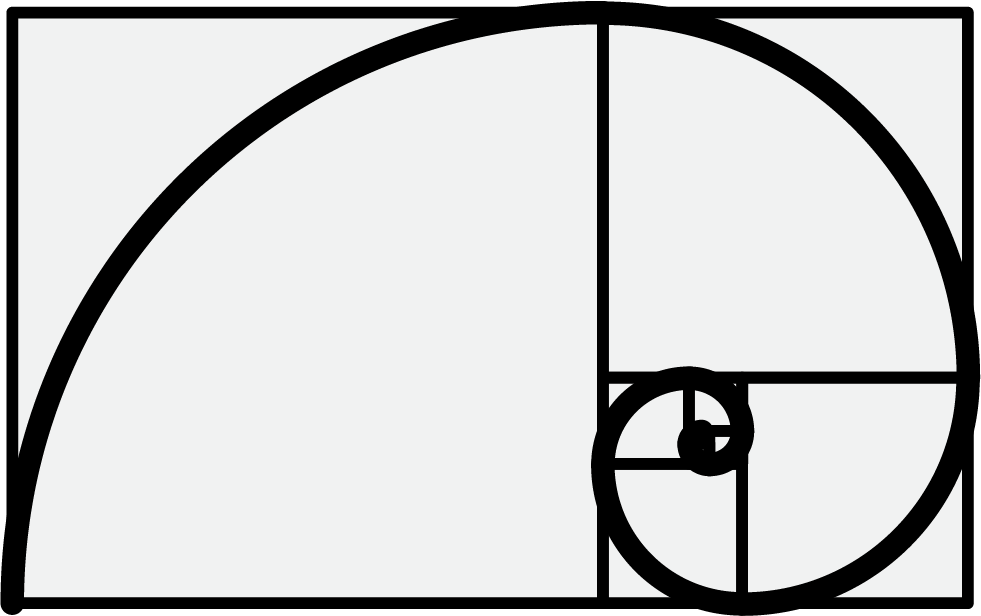
\includegraphics[height=0.75cm]{../../../AAA_template_latex_settings/pwr-control_logo_doc.png}}
\rfoot{\small Rev.~00}
\geometry{left=2.0cm, right=2.0cm}
\usepackage{pdflscape}
\usepackage{afterpage}
\newcolumntype{R}[1]{>{\RaggedRight\arraybackslash}p{#1}}
\usetikzlibrary{shapes.geometric}

\sisetup{per-mode=symbol,range-phrase={\text{--}},range-units=single}
\setlist{nosep}
\setlength{\parindent}{0pt}
\setlength{\parskip}{3pt}
\allowdisplaybreaks

% --- shorthand ---
\newcommand{\ts}{t_s}
\newcommand{\wo}{\omega_0}
\newcommand{\wres}{\omega_r}
\newcommand{\kmod}{k_{mod}}
\newcommand{\kpi}{k_{p,i}}
\newcommand{\kii}{k_{i,i}}
\newcommand{\kpu}{k_{p,u}}
\newcommand{\kiu}{k_{i,u}}
\newcommand{\kpn}{k_{p,n}}
\newcommand{\kin}{k_{i,n}}
\newcommand{\jj}{\mathrm{j}}
\newcommand{\ee}{\mathrm{e}}
\newcommand{\dif}{\mathrm{d}}
\newcommand{\pu}{\,\mathrm{pu}}
\newcommand{\code}[1]{\texttt{#1}}
\newcommand{\uhat}{\hat{u}}
\newcommand{\vhat}{\hat{v}}
\renewcommand{\Re}{\operatorname{Re}}
\renewcommand{\Im}{\operatorname{Im}}

% =============================================================
%  DOCUMENT DATA (title page: AAA_template_latex_settings/titlepage.tex)
% =============================================================
\newcommand{\DocCategory}{Technical Note}
\newcommand{\DocField}{Power Electronics and Control Systems}
\newcommand{\DocTitle}{%
	{\fontsize{20}{24}\selectfont\bfseries Grid-Forming Control in the Synchronous dq Frame:} \\[12pt]
	{\fontsize{16}{26}\selectfont\bfseries structure, continuous-time design \\[8pt] and discrete implementation}
}
\newcommand{\DocSubtitle}{The controller of the library block \texttt{grid\_forming\_dqctrl} (\texttt{afe\_dq\_ctrl\_pwm}): \\[6pt] voltage loops on the positive and negative sequence, FHT sequence separation, \\[6pt] PI plus resonant current loop, and where the exact discretization is required}
\newcommand{\DocAuthor}{Davide Bagnara}
\newcommand{\DocRevision}{00}
\newcommand{\DocDate}{October 2026}
\newcommand{\DocAbstract}{%
This note documents the control of the grid-forming three-phase converter implemented in the MATLAB Function \texttt{afe\_dq\_ctrl\_pwm} of the library block \texttt{grid\_forming\_dqctrl} (used by the VFC0 test bench at \SI{16.7}{Hz}) and, with the same structure, in the Simulink study model \texttt{grid\_forming\_dq.slx} (\SI{400}{V}, \SI{250}{kW}, \SI{50}{Hz}). The converter forms the voltage of an islanded load through its LCL filter and a coupling transformer: a free-running phase generator fixes the frequency, a first harmonic tracker (FHT, a resonant observer) on the $\alpha\beta$ terminal voltage separates the positive and the negative sequence, a vector PI in the positive frame regulates the positive-sequence voltage, a second vector PI in the negative frame drives the negative-sequence voltage to zero, and the two current references, the second rotated by $-2\theta$ into the positive frame, are tracked by a vector PI on the converter current with a resonant term at $2\omega_0$ on each axis. The note gives the structure block by block, the continuous-time analysis of every loop with complex space vectors (current loop, pole-displacement rule of the resonant term and the design rule $k_r = 2k_{i,i}$, closed-form observer gains and sequence-separation accuracy of the FHT, output impedance of the grid-forming voltage loops) and the discrete implementation operation by operation at the control period $t_s = 1/(2f_{pwm})$. It states where the discretization must be exact: the resonant internal model (poles on the unit circle at exactly $2\omega_0 t_s$, semi-implicit form with $a = 2\sin(\omega_r t_s/2)$ or zero-order hold; the forward Euler form of the library object is unstable at \SI{100}{Hz} and \SI{125}{\micro s}), the internal model of the FHT with $\delta = 0$ and the quadrature output taken at the same instant as the in-phase one, while the PI integrators and the frame rotations need no special care. A companion Python script reproduces every number and figure.
}
\newcommand{\RevisionHistory}{%
	00 & October 2026 & First issue. & \DocAuthor \\
}
\newcommand{\MetaLabelA}{Project Repository}
\newcommand{\MetaValueAUrl}{https://github.com/pwr-control/library.git}
\newcommand{\MetaValueALabel}{library.git (masked\_models/grid\_forming)}
\newcommand{\MetaLabelB}{Framework}
\newcommand{\MetaValueB}{MATLAB/Simulink/Simscape; Python 3 (\texttt{grid\_forming\_control\_analysis.py})}

\begin{document}
% =============================================================
%  pwr-control LaTeX template - FRONTESPIZIO
%
%  Da richiamare come prima istruzione dopo \begin{document}:
%      \input{../../AAA_template_latex_settings/titlepage}
%
%  Il documento deve definire prima di \begin{document}:
%      \DocCategory   categoria del documento
%      \DocField      area tecnica
%      \DocTitle      titolo (una o due righe)
%      \DocSubtitle   sottotitolo
%      \DocAuthor     autore/i, separati da virgola
%      \DocRevision   numero di revisione corrente (es. 00)
%      \DocDate       data della revisione corrente
%      \DocAbstract   abstract
%      \RevisionHistory  righe della tabella di revisione, nel formato
%                        Rev. & Date & Description & Authors \\
%      \MetaLabelA \MetaValueAUrl \MetaValueALabel
%      \MetaLabelB \MetaValueB
% =============================================================

\providecommand{\DocCategory}{Technical Research Report}
\providecommand{\DocField}{Power Electronics and Control Systems}
\providecommand{\DocSubtitle}{}
\providecommand{\DocRevision}{00}
\providecommand{\DocAbstract}{}
\providecommand{\RevisionHistory}{%
	\DocRevision & \DocDate & First issue. & \DocAuthor \\
}

\titlepage

% ---- Intestazione centrata ----
\begin{center}
	{\Large\scshape \DocCategory}\\[8pt]
	{\large\scshape \DocField}
\end{center}

\vspace{30pt plus 4pt minus 14pt}
\noindent\rule{\linewidth}{0.8pt}

% ---- Titolo ----
\begin{center}
	\DocTitle
\end{center}

\vspace{4pt}
\noindent\rule{\linewidth}{2.2pt}

% ---- Sottotitolo ----
\begin{center}
	\begin{onehalfspace}
		{\large\itshape \DocSubtitle}
	\end{onehalfspace}
\end{center}

% ---- Authors / Revision / Date ----
\vspace{30pt plus 4pt minus 14pt}

\noindent
\begin{minipage}[t]{0.46\linewidth}
	\raggedright
	\textbf{Authors:}\\[2pt]
	\DocAuthor
\end{minipage}%
\hfill
\begin{minipage}[t]{0.22\linewidth}
	\centering
	\textbf{Revision:}\\[2pt]
	\DocRevision
\end{minipage}%
\hfill
\begin{minipage}[t]{0.30\linewidth}
	\raggedleft
	\textbf{Date:}\\[2pt]
	\DocDate
\end{minipage}

\vspace{10pt}
\noindent\rule{\linewidth}{0.8pt}

% ---- Abstract ----
\vspace{24pt plus 4pt minus 12pt}

\begin{center}
	\begin{minipage}{0.88\linewidth}
		\footnotesize
		\begin{onehalfspace}
			\textbf{Abstract:} \DocAbstract
		\end{onehalfspace}
	\end{minipage}
\end{center}

\vfill

% ---- Revision history ----
\begin{center}
	\begin{minipage}{0.96\linewidth}
		\centering
		{\footnotesize\scshape Revision history}\\[6pt]
		{\footnotesize
			\begin{tabular}{@{}cl>{\raggedright\arraybackslash}p{0.36\linewidth}>{\raggedright\arraybackslash}p{0.28\linewidth}@{}}
				\toprule
				\textbf{Rev.} & \textbf{Date} & \textbf{Description} & \textbf{Authors} \\
				\midrule
				\RevisionHistory
				\bottomrule
			\end{tabular}}
	\end{minipage}
\end{center}

\vspace{18pt plus 4pt minus 10pt}

% ---- Metadati in fondo ----
\noindent
\begin{tabular}{@{} r @{\quad} l @{}}
	\textsc{\MetaLabelA:} & {\href{\MetaValueAUrl}{\MetaValueALabel}} \\[3pt]
	\textsc{\MetaLabelB:} & {\MetaValueB}       \\[3pt]
\end{tabular}

% =============================================================
%  Fine frontespizio
% =============================================================
\newpage
\pagenumbering{arabic}
\setcounter{page}{1}

\tableofcontents
\newpage
\begin{onehalfspace}

% =====================================================================================================
\section{Scope}
\label{sec:scope}

The grid-forming converter considered here is a two-level three-phase voltage-source converter with an LCL output filter feeding, through a coupling transformer, an islanded load that can be unbalanced (a single-phase load on one secondary, for instance). The converter alone fixes the amplitude and the frequency of the load voltage. The control is implemented twice with the same structure and the same signal names:
\begin{itemize}
\item in the MATLAB Function \code{afe\_dq\_ctrl\_pwm} of the library block \code{grid\_forming\_dqctrl} (\path{library/masked_models/grid_forming}), which holds the control and the PWM of one converter in one block, with a master/slave mode for converters in parallel and the negative-sequence compensator (\code{nsc\_enable = 1}); it is the block used by the model of the VFC0 test bench (\SI{16.7}{Hz}, two converters GFM1 master and GFM2 slave, \SI{2.5}{kHz} double update);
\item in the Simulink model \code{grid\_forming\_dq.slx} (\path{foundations_of_power_electronics/grid_forming/single_phase_load} of modelization-and-control), the study model of the same control at \SI{50}{Hz} with Simulink blocks and C-Caller blocks of the library (\SI{400}{V}, \SI{250}{kW}, \SI{4}{kHz} double update, Dyn11 \SI{1}{MVA} transformer, RL load with \SI{\pm 10}{\percent} unbalance), where the loops were tuned and checked.
\end{itemize}
The note describes the control, not the power stage: Sect.~\ref{sec:system} fixes the notation and the plant model, Sect.~\ref{sec:structure} walks through the control structure, Sect.~\ref{sec:analysis} is the continuous-time analysis of each loop, Sect.~\ref{sec:discrete} the discrete implementation operation by operation with the discussion of where the discretization must be exact, Sect.~\ref{sec:verification} the numerical verification and Sect.~\ref{sec:parameters} the parameters of the two applications. Every number of the note comes from the companion script \code{grid\_forming\_control\_analysis.py}, a linear model of the \SI{50}{Hz} study model (plant, delays and controller written as in the code); the plant-dependent figures therefore refer to that model, while the controller equations, the discretization results and the FHT figures hold for both applications and are given for both.

% =====================================================================================================
\section{System, notation and plant model}
\label{sec:system}

\subsection{Power stage and per-unit base}

Fig.~\ref{fig:overview} (right) shows the power stage: the DC link $u_{dc}$, the two-level bridge, the converter-side reactor $L_1$ (resistance $R_1$), the star-connected filter capacitor $C_F$ with its series resistance $R_{CF}$, the grid-side reactor $L_2$ ($R_2$) and the terminals, connected to a primary of the coupling transformer. The control measures the converter current $i_s$ (positive out of the bridge), the terminal voltage $u_g$ (phase voltages, zero sequence removed) and $u_{dc}$; the grid current $i_g$ is acquired for the log only.

All the signals of the control are per unit: $u_{bez} = \sqrt{2/3}\,U_{n}$ is the peak of the nominal phase voltage ($U_n$ line-to-line) and $i_{bez} = \sqrt{2}\,I_n$ the peak of the nominal phase current, $z_{bez} = u_{bez}/i_{bez}$. Inductances and capacitances in per unit are times: $L' = L/z_{bez}$ and $C' = C\,z_{bez}$ in seconds. The modulation index vector $\vec m$ is the output of the current controller; the space-vector modulator maps $|\vec m| = 1$ to the limit of the linear range, i.e. to a phase-voltage amplitude $u_{dc}/\sqrt3$, so the converter voltage in per unit is
\begin{equation}
\vec u_{conv} = \kmod\,\vec m, \qquad \kmod = \frac{u_{dc}}{\sqrt3\,u_{bez}},
\label{eq:kmod}
\end{equation}
$\kmod = 1.167$ for the study model ($u_{dc} = \SI{660}{V}$, $u_{bez} = \SI{326.6}{V}$). The DC-link voltage is not compensated in the modulation: $\kmod$ is a gain of the plant.

\subsection{Space vectors, frames and sequences}

The amplitude-invariant Clarke transformation gives the stationary components $x_\alpha = \tfrac23(x_a - \tfrac12 x_b - \tfrac12 x_c)$, $x_\beta = (x_b - x_c)/\sqrt3$, written as the complex space vector $\vec x = x_\alpha + \jj x_\beta$. The positive synchronous frame $\xi\eta$ rotates with the angle $\theta$ of the phase generator,
\begin{equation}
\vec x_{\xi\eta} = \vec x_{\alpha\beta}\,\ee^{-\jj\theta}, \qquad
x_\xi = x_\alpha\cos\theta + x_\beta\sin\theta, \quad x_\eta = -x_\alpha\sin\theta + x_\beta\cos\theta,
\label{eq:posframe}
\end{equation}
the negative frame rotates the other way, $\vec x^{(n)} = \vec x_{\alpha\beta}\,\ee^{+\jj\theta}$. A balanced positive-sequence set at $\wo = 2\pi f_0$ is a vector turning at $+\wo$, constant in the positive frame; a negative-sequence set (Fortescue \cite{fortescue1918}) turns at $-\wo$, is constant in the negative frame and turns at $-2\wo$ in the positive frame. The zero sequence does not enter the space vector. With $\theta$ advancing at exactly $\wo$ every balanced quantity of the fundamental is a DC value in its frame, and a vector PI (the same real gains $k_p$, $k_i$ on the two axes, i.e. a real transfer function acting on the complex error) regulates it without steady-state error. Throughout the note the loops are written with complex space vectors in the positive frame: the plant is balanced, so each loop is a complex-coefficient single-input single-output system \cite{harnefors2007}, a sinusoid at $f$ in the stationary frame appears at $f - f_0$ and the negative sequence of the fundamental at $-2f_0$.

\subsection{Timing of the digital control}
\label{sec:timing}

The carrier is triangular at $f_{pwm}$ and the control runs twice per carrier period (double update), at its top and at its bottom (the TRGO flag): the control period is $\ts = 1/(2f_{pwm})$, \SI{200}{\micro s} for VFC0 and \SI{125}{\micro s} for the study model. The acquisitions are sampled on the TRGO and quantized ($q = 2^{-11}\pu$); the control step $k$ uses the samples taken at step $k-1$ (one-step acquisition delay, the model of the conversion and computation time) and the duties it computes are loaded at once and act over the following half period. The loop therefore sees the usual delay of a digital PWM converter, one step of computation plus the half-step average of the hold \cite{buso2015}:
\begin{equation}
D(s) = \ee^{-1.5\,\ts s}.
\label{eq:delay}
\end{equation}
In discrete time the delay is one sample ($z^{-1}$) in front of a zero-order hold; this is how the companion script models it.

\subsection{Plant model}
\label{sec:plant}

In the stationary frame, with complex vectors and per-unit quantities, the LCL filter with the passive network beyond the capacitor node (grid-side reactor, transformer leakage, load: $L_g = L_2 + L_\sigma + L_{load}$, $R_g = R_2 + R_\sigma + R_{load}$) is
\begin{align}
L_1'\,\frac{\dif\vec i_1}{\dif t} &= \kmod\,\vec m - \vec u_c - R_{CF}'(\vec i_1 - \vec i_2) - R_1'\,\vec i_1, \nonumber\\
C_F'\,\frac{\dif\vec u_c}{\dif t} &= \vec i_1 - \vec i_2 - \vec i_d, \label{eq:plant}\\
L_g'\,\frac{\dif\vec i_2}{\dif t} &= \vec u_c + R_{CF}'(\vec i_1 - \vec i_2) - R_g'\,\vec i_2, \nonumber
\end{align}
where $\vec i_d$ is a current drawn at the capacitor node that represents the unbalanced part of the load (a negative-sequence current at $-\wo$, i.e. $-2\wo$ in the positive frame), and the terminal voltage is $\vec u_g = \vec u_c + R_{CF}'(\vec i_1 - \vec i_2) - L_2'\,\dif\vec i_2/\dif t - R_2'\,\vec i_2$. In the positive frame, $\vec x = \vec{\tilde x}\,\ee^{\jj\theta}$ with $\dot\theta = \wo$, every derivative gains the term $\jj\wo\vec{\tilde x}$: the state matrix becomes $A - \jj\wo I$ and every transfer function of the stationary frame is evaluated at $s + \jj\wo$ \cite{harnefors2007}. Table~\ref{tab:plant} gives the values of the study model. The LCL resonance is at \SI{1045}{Hz} with a stiff grid at the terminals and at about \SI{600}{Hz} with the transformer and the load of the model, in both cases below the critical frequency $f_s/6 = \SI{1333}{Hz}$ of the converter-current feedback \cite{parker2014}, so the current loop damps the resonance (closed-loop LCL modes with $\sigma \approx \SI{-800}{s^{-1}}$ in Sect.~\ref{sec:verification}).

\begin{table}[htb]
\centering\small\setlength{\tabcolsep}{4pt}
\caption{Plant of the study model (\SI{400}{V}, \SI{250}{kW}, \SI{50}{Hz}; $z_{bez} = \SI{0.576}{\ohm}$).}
\label{tab:plant}
\begin{tabular}{@{}lll@{}}
\toprule
element & value & per unit \\
\midrule
converter reactor $L_1$, $R_1$ & \SI{330}{\micro H}, \SI{2.6}{m\ohm} & $L_1' = \SI{0.573}{ms}$, $R_1' = 0.0045$ \\
filter capacitor $C_F$, $R_{CF}$ & \SI{360}{\micro F}, \SI{50}{m\ohm} & $C_F' = \SI{0.207}{ms}$ ($\wo C_F' = 0.065$), $R_{CF}' = 0.087$ \\
grid reactor $L_2$, $R_2$ & \SI{80}{\micro H}, \SI{0.6}{m\ohm} & $L_2' = \SI{0.139}{ms}$ \\
transformer Dyn11 \SI{1}{MVA}, $u_{cc}$ \SI{5}{\percent} & $L_\sigma = \SI{25.5}{\micro H}$ & \\
RL load (phase mean, primary side) & \SI{0.556}{\ohm}, \SI{0.98}{mH} & $R_{load}' = 0.965$ \\
total beyond the capacitor $L_g$, $R_g$ & & $L_g' = \SI{1.884}{ms}$, $R_g' = 0.980$ \\
modulation gain, control period & $u_{dc} = \SI{660}{V}$, $f_{pwm} = \SI{4}{kHz}$ & $\kmod = 1.167$, $\ts = \SI{125}{\micro s}$ \\
\bottomrule
\end{tabular}
\end{table}

% =====================================================================================================
\section{Control structure}
\label{sec:structure}

\subsection{Overview}

Fig.~\ref{fig:overview} is the block diagram of the control as coded in \code{afe\_dq\_ctrl\_pwm} for the VFC0 test bench (signal names as in the code, column indices of the log in brackets); Fig.~\ref{fig:linear} is the equivalent linear model used in the analysis. The chain, executed once per control step, is:
\afterpage{%
\begin{landscape}
\begin{figure}[p]
\centering
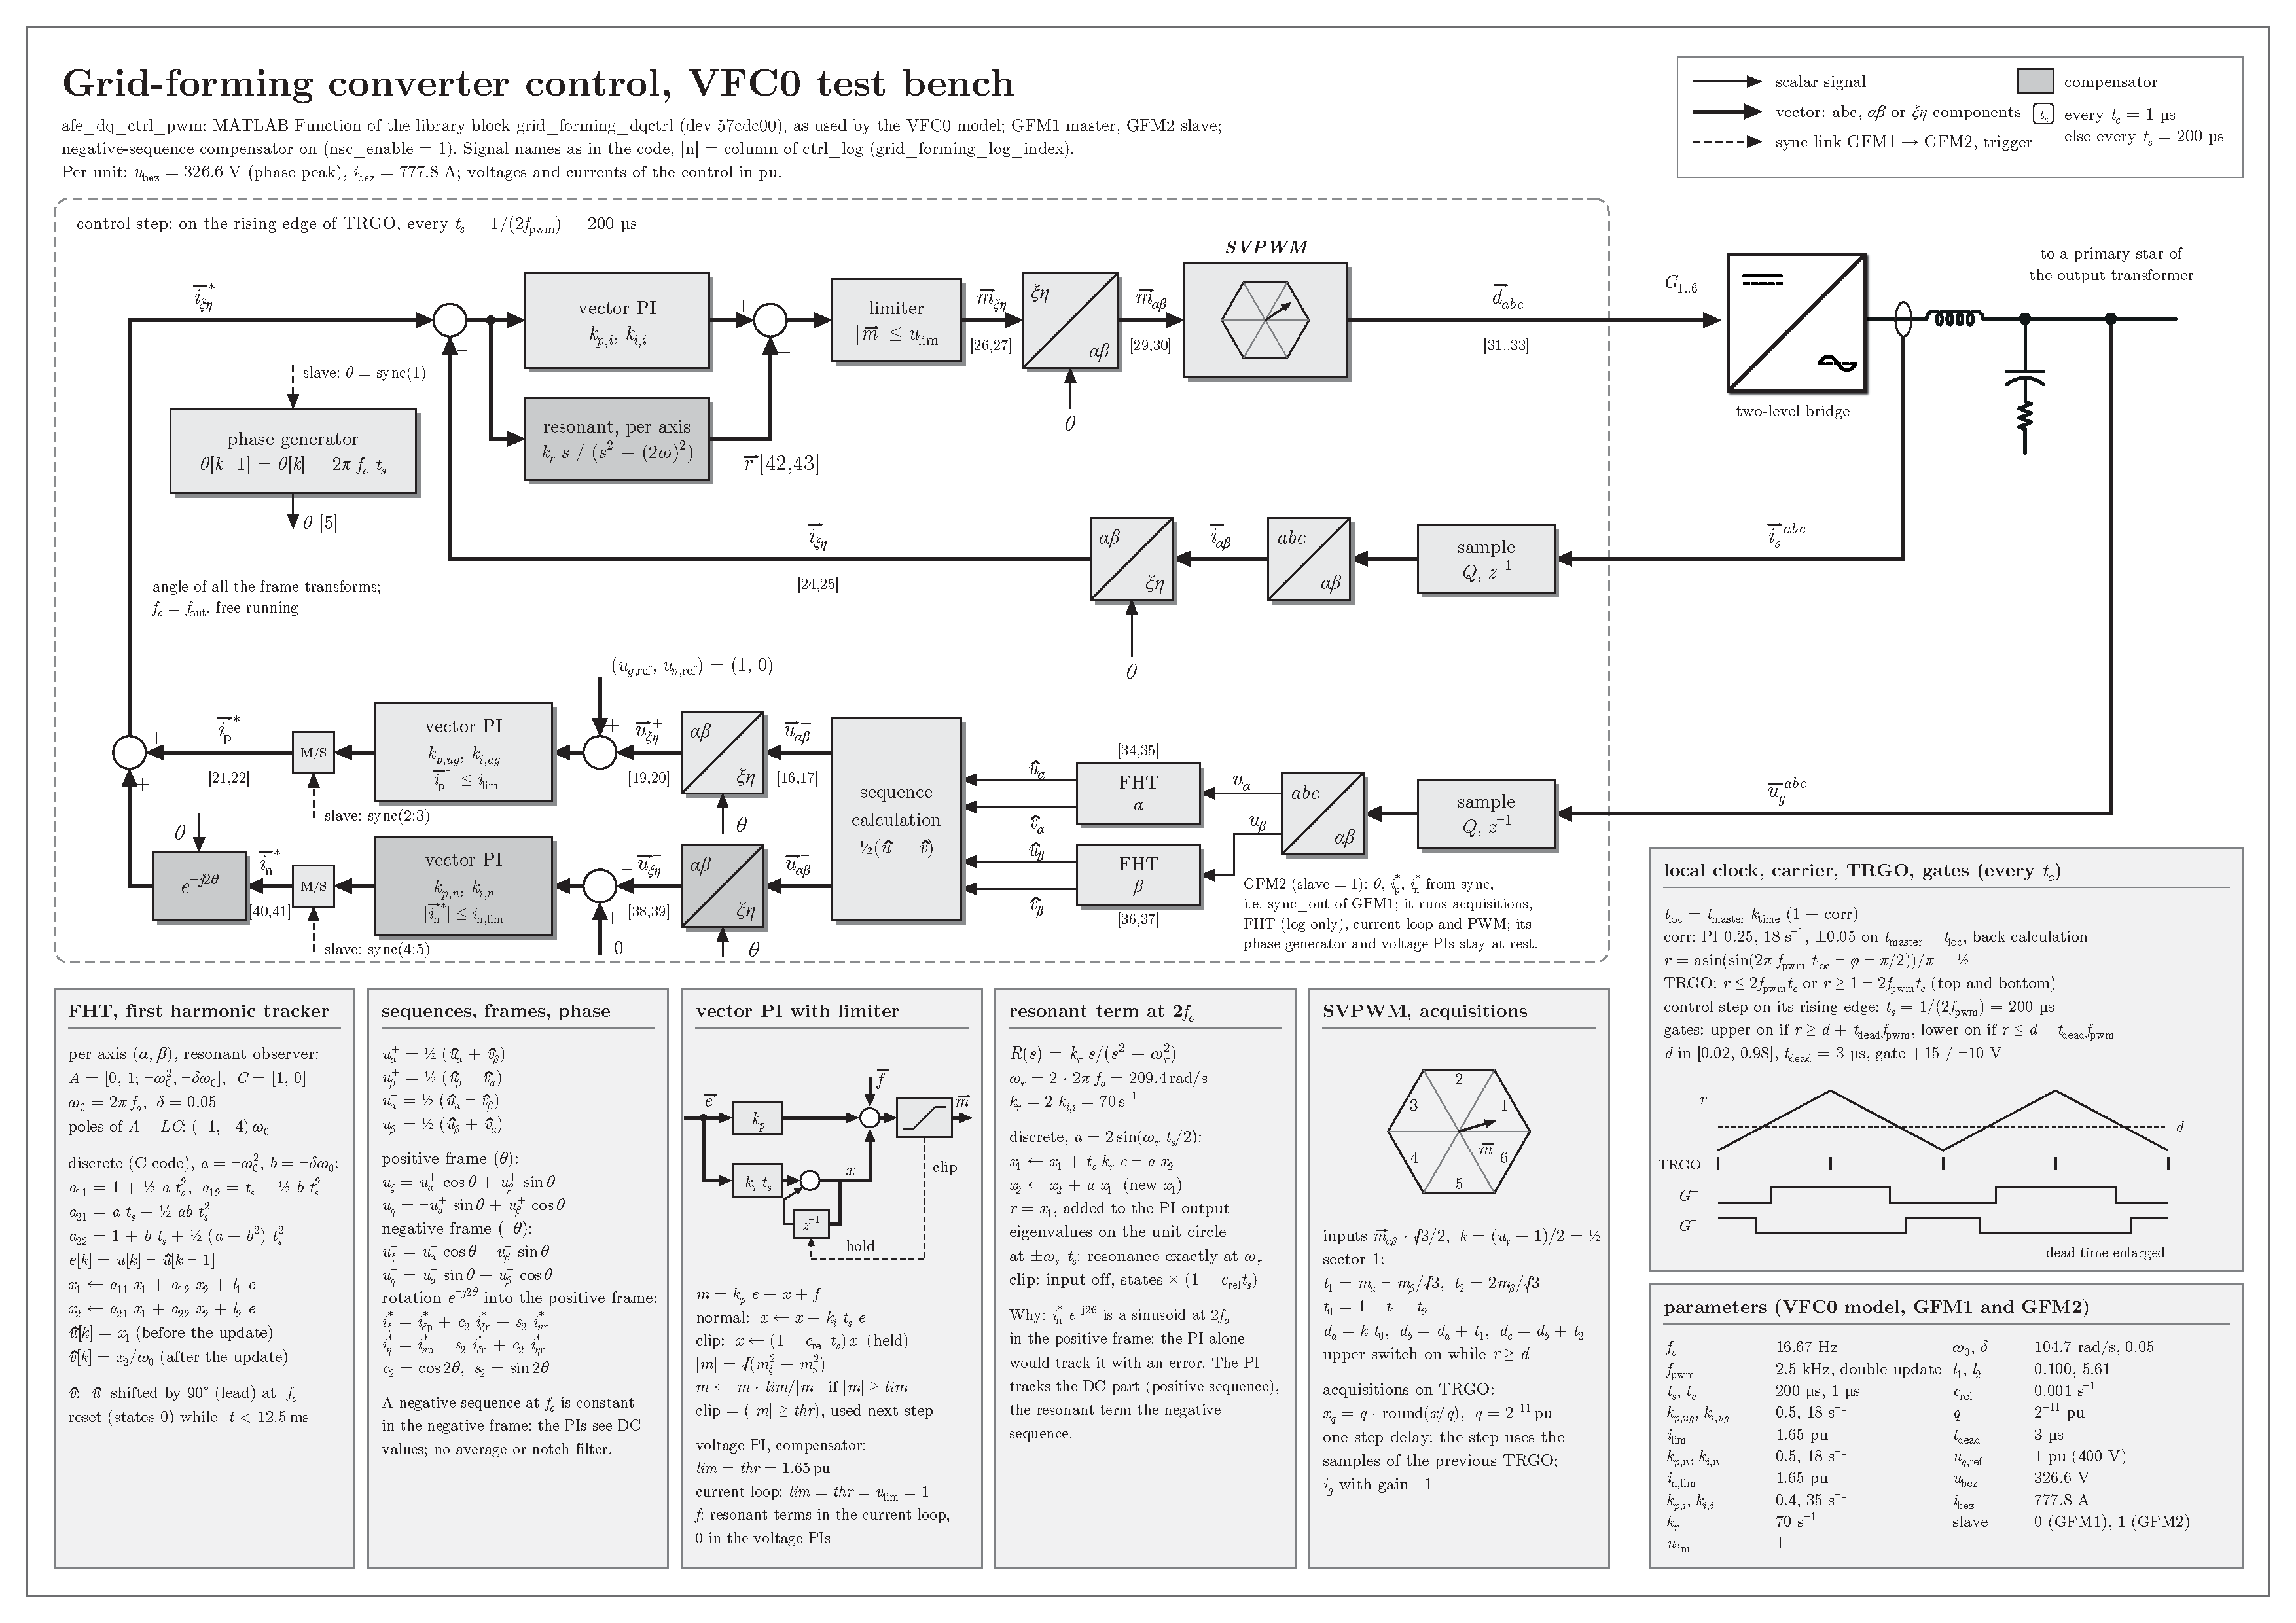
\includegraphics[width=0.98\linewidth]{figures/grid_forming_ctrl_vfc0.pdf}
\caption{Control of the grid-forming converter as implemented in \code{afe\_dq\_ctrl\_pwm} (library block \code{grid\_forming\_dqctrl}, dev 57cdc00) for the VFC0 test bench, with the negative-sequence compensator. Diagram \code{grid\_forming\_ctrl\_ver\_ii} of the adobe-illustrator-diagrams repository (\code{ai\_diagrams/AAA\_projects/VFC0}).}
\label{fig:overview}
\end{figure}
\end{landscape}
}
\begin{enumerate}
\item \textbf{Acquisitions.} $u_g$, $i_s$, $i_g$, $u_{dc}$ sampled at the TRGO, quantized, used at the next step.
\item \textbf{Sequence separation.} $u_g$ to $\alpha\beta$; one FHT per axis gives the fundamental $\uhat_\alpha$, $\uhat_\beta$ and its quadrature $\vhat_\alpha$, $\vhat_\beta$ (\SI{90}{\degree} lead at $f_0$); the positive and negative sequence of the fundamental follow from the quadrature-signal method of \cite{rodriguez2006}:
\begin{equation}
\vec u^{+} = \tfrac12(\vec{\uhat} - \jj\vec{\vhat}), \qquad \vec u^{-} = \tfrac12(\vec{\uhat} + \jj\vec{\vhat}),
\label{eq:sequences}
\end{equation}
i.e. $u^+_\alpha = \tfrac12(\uhat_\alpha + \vhat_\beta)$, $u^+_\beta = \tfrac12(\uhat_\beta - \vhat_\alpha)$, $u^-_\alpha = \tfrac12(\uhat_\alpha - \vhat_\beta)$, $u^-_\beta = \tfrac12(\uhat_\beta + \vhat_\alpha)$.
\item \textbf{Phase generator.} $\theta$ advances by $2\pi f_0\ts$ per step, free running: the converter imposes the frequency $f_0$. It is the angle of every frame transformation.
\item \textbf{Positive-sequence voltage loop.} $\vec u^{+}$ in the positive frame; vector PI ($\kpu$, $\kiu$) on $(u^*_{\xi} - u^+_\xi,\ u^*_\eta - u^+_\eta)$ with $(u^*_\xi, u^*_\eta) = (1, 0)$; output $\vec i^*_p$, limited to $|\vec i^*_p| \le i_{lim}$.
\item \textbf{Negative-sequence voltage loop (compensator).} $\vec u^{-}$ in the negative frame (angle $-\theta$), where a negative sequence at $f_0$ is a DC value; vector PI ($\kpn$, $\kin$) with reference zero; output $\vec i^*_n$ in the negative frame, limited to $i_{n,lim}$.
\item \textbf{Current references.} $\vec i^*_n$ rotated into the positive frame by $\ee^{-\jj 2\theta}$ (a vector turning at $-2\wo$, a sinusoid at $2f_0$ on each axis) and added to $\vec i^*_p$.
\item \textbf{Current loop.} Converter current $i_s$ in the positive frame; vector PI ($\kpi$, $\kii$) plus, on each axis, the resonant term $R(s) = k_r s/(s^2 + \wres^2)$ at $\wres = 2\wo$; the sum is the modulation vector $\vec m$, limited to the unit circle.
\item \textbf{Modulation.} $\vec m$ back to $\alpha\beta$ (angle $+\theta$), space-vector PWM (duties $d_{abc}$), gate commands with the dead time every $t_c$.
\end{enumerate}
No voltage feed-forward is used in the current loop and no load-current feed-forward in the voltage loops: all the current the load draws is built up by the integrators of the voltage loops. The limiters raise a clip flag that, at the next step, stops the integrators (and the resonant terms) of the loop that clipped (Sect.~\ref{sec:limits}).

In the master/slave mode (converters on separate primaries of one transformer) the slave takes $\theta$, $\vec i^*_p$ and $\vec i^*_n$ from the master through the \code{sync} link and runs only its acquisitions, its current loop and its PWM, so that identical converters carry the same current in per unit of their own base; its FHT runs for the log only and its voltage PIs stay at rest.


\subsection{Linear model of the loops}

\begin{figure}[htb]
\centering
\begin{tikzpicture}[>=Latex, font=\footnotesize,
  blk/.style={draw, minimum height=7mm, minimum width=11mm, inner sep=3pt, align=center, fill=gray!8},
  sum/.style={draw, circle, minimum size=4mm, inner sep=0pt},
  lbl/.style={inner sep=1.5pt}]
% positive-sequence voltage loop
\node[sum] (s1) at (0,0) {};
\node[lbl, left=3mm of s1] (uref) {$\vec u^{*} = 1$};
\draw[->] (uref) -- (s1);
\node[blk] (piu) at (1.9,0) {$\kpu + \tfrac{\kiu}{s}$};
\draw[->] (s1) -- (piu);
\node[sum] (s2) at (3.9,0) {};
\draw[->] (piu) -- node[above, lbl] {$\vec i^*_p$} (s2);
% negative-sequence voltage loop, written in the positive frame
\node[sum] (s1n) at (1.0,-1.9) {};
\node[lbl, left=3mm of s1n] (nref) {$0$};
\draw[->] (nref) -- (s1n);
\node[blk] (pin) at (2.6,-1.9) {$\kpn + \tfrac{\kin}{s - \jj 2\wo}$ \\ {\scriptsize negative-sequence PI}};
\draw[->] (s1n) -- (pin);
\draw[->] (pin.east) -| (s2.south);
\node[lbl, left] at (3.8,-1.0) {$\vec i^*_n\,\ee^{-\jj2\theta}$};
% current loop
\node[sum] (s3) at (4.8,0) {};
\draw[->] (s2) -- node[above, lbl] {$\vec i^*$} (s3);
\node[blk] (ci) at (7.0,0) {$\kpi + \tfrac{\kii}{s} + \tfrac{k_r s}{s^2 + \wres^2}$};
\draw[->] (s3) -- node[above, lbl] {$\vec e_i$} (ci);
\node[blk] (del) at (9.9,0) {$\kmod\,\ee^{-1.5\ts s}$};
\draw[->] (ci) -- node[above, lbl] {$\vec m$} (del);
\node[blk, minimum width=22mm] (pl) at (12.3,0) {LCL + load \\ $A - \jj\wo I$};
\draw[->] (del) -- (pl);
\node[lbl] (out) at (14.8,0) {$\vec i_1$, $\vec u_g$};
\draw[->] (pl) -- (out);
\node[lbl, above=2.5mm of pl] (id) {$\vec i_d$ (unbalance)};
\draw[->] (id) -- (pl);
% feedbacks
\draw[->] (13.6,0) |- (4.8,-1.0) -- (s3.south);
\node[lbl, above] at (9.0,-1.0) {$\vec i_1$};
\node[blk, minimum width=22mm] (fht) at (12.3,-3.1) {FHT $\alpha\beta$ \\ $\vec u^{\pm} = \tfrac12(\vec{\uhat} \mp \jj\vec{\vhat})$};
\draw[->] (13.9,0) |- (fht.east);
\node[lbl, right] at (13.9,-1.6) {$\vec u_g$};
\draw[->] (fht.west) -| (s1n.south);
\node[lbl, above] at (7.0,-3.1) {$\vec u^{-}$};
\draw[->] (fht.south) |- (0,-3.9) -- (s1.south);
\node[lbl, above] at (7.0,-3.9) {$\vec u^{+}$};
\node[lbl, above left=-0.5mm and -0.5mm of s1] {$+$};
\node[lbl, below right=-0.5mm and -0.5mm of s1] {$-$};
\node[lbl, below right=-0.5mm and -0.5mm of s1n] {$-$};
\node[lbl, below right=-0.5mm and -0.5mm of s3] {$-$};
\end{tikzpicture}
\caption{Linear model of the loops in the positive dq frame (complex space vectors). The negative-sequence PI acts in the negative frame; written in the positive frame its integrator pole sits at $s = -\jj 2\wo$, its input is the negative-sequence estimate of the FHT (reference zero) and its output is the rotated reference $\vec i^*_n\,\ee^{-\jj 2\theta}$.}
\label{fig:linear}
\end{figure}

% =====================================================================================================
\section{Continuous-time analysis}
\label{sec:analysis}

\subsection{Current loop: vector PI}
\label{sec:currentloop}

Without the capacitor-voltage feed-forward the plant seen by the current controller depends on everything beyond $L_1$. Two views are useful. For the \emph{design} of the gains the capacitor voltage is treated as a disturbance,
\begin{equation}
P_{i}(s) \simeq \frac{\kmod}{L_1'(s + \jj\wo) + R_1'} \simeq \frac{\kmod}{L_1' s} \quad (|s| \gg \wo),
\label{eq:plant_design}
\end{equation}
and with the PI $C_i(s) = \kpi + \kii/s$ and the delay (\ref{eq:delay}) the crossover and the phase margin are
\begin{equation}
\omega_c \simeq \frac{\kpi\kmod}{L_1'}, \qquad
\varphi_m \simeq \SI{90}{\degree} - 1.5\,\omega_c\ts\,\frac{180}{\pi} - \arctan\frac{\kii}{\kpi\omega_c}.
\label{eq:pm}
\end{equation}
For the study model ($\kpi = 0.75$, $\kii = \SI{35}{s^{-1}}$): $\omega_c = \SI{1527}{rad/s}$ (\SI{243}{Hz}, \SI{19}{\percent} of $f_s/4$), delay phase \SI{16.4}{\degree}, PI zero at $\kii/\kpi = \SI{46.7}{rad/s}$ (\SI{7.4}{Hz}), $\varphi_m = \SI{72}{\degree}$. The uncompensated cross-coupling $\jj\wo L_1'$ is $\wo/\omega_c = 0.2$ of the plant at the crossover and is left to the loop.

For the \emph{behaviour at low frequency}, where the capacitor is an open circuit, the converter sees $L_1 + L_g$ and $R_1 + R_g$, i.e. the load: in the positive frame the loaded plant at DC is $|P(0)| = \kmod/|R_1' + R_g' + \jj\wo(L_1' + L_g')| = 0.909$ and the proportional loop gain is only $\kpi|P(0)| = 0.68$, so that the proportional action alone would leave \SI{58}{\percent} of a DC error ($T_P(0) = \kpi P/(1 + \kpi P) = 0.42$). The integrator removes it with the closed-loop pole
\begin{equation}
s_I \simeq -\kii\,\frac{T_P(0)}{\kpi} \;=\; -\kii\,\frac{P(0)}{1 + \kpi P(0)},
\label{eq:integrator_pole}
\end{equation}
$\SI{-20}{s^{-1}}$ with these numbers ($\SI{-18.7}{s^{-1}}$ from the full model of Sect.~\ref{sec:verification}). The same loop at the frequency of the negative sequence, $s = -\jj 2\wo$, where $|P| = 0.909$ as well, has the closed-loop gain $T_{PI}(-\jj2\wo) = 0.44\,\angle\SI{+23}{\degree}$: a negative-sequence current reference is tracked by the PI alone with a \SI{56}{\percent} amplitude error and a \SI{23}{\degree} phase error. This is the motivation of the resonant term.

\subsection{Negative sequence in the positive frame: the resonant term}
\label{sec:resonant}

A negative-sequence current reference $\vec i^*_n\,\ee^{-\jj2\theta}$ is a vector turning at $-2\wo$ in the positive frame, a sinusoid at $\wres = 2\wo$ on each axis. By the internal model principle the loop tracks it with zero steady-state error only if the controller has poles at $\pm\jj\wres$ \cite{zmood2003, teodorescu2006}; the term added on each axis in parallel with the PI,
\begin{equation}
R(s) = \frac{k_r s}{s^2 + \wres^2} = \frac{k_r}{2}\left(\frac{1}{s - \jj\wres} + \frac{1}{s + \jj\wres}\right),
\label{eq:resonant}
\end{equation}
is the sum of two complex integrators of gain $k_r/2$ \cite{liserre2006}. Acting on the complex error with real coefficients it provides infinite gain at $s = -\jj\wres$, the negative sequence of the fundamental, and at $s = +\jj\wres$, the positive-sequence third harmonic in the stationary frame, which is not needed but harmless. (A single-sided complex term $k_r/(s + \jj\wres)$, obtained by cross-coupling the two axes, would act on the negative sequence only; it is not implemented.)

\paragraph{Pole displacement rule.} Near $s = \jj\wres$ the resonant term is $R(s) \simeq (k_r/2)/(s - \jj\wres)$ and the characteristic equation $1 + [C_i(s) + R(s)]\,P(s)D(s) = 0$ of the loop becomes $(s - \jj\wres)\,[1 + L_{PI}(\jj\wres)] + (k_r/2)\,P D(\jj\wres) = 0$, with $L_{PI} = C_i P D$ the loop gain of the PI alone, so that the closed-loop pole born from the resonance sits at
\begin{equation}
s_r \simeq \jj\wres - \frac{k_r}{2}\,\frac{P D(\jj\wres)}{1 + L_{PI}(\jj\wres)} = \jj\wres - \frac{k_r}{2}\,\frac{T_{PI}(\jj\wres)}{C_i(\jj\wres)},
\label{eq:pole_rule}
\end{equation}
and likewise at $-\jj\wres$. $T_{PI} = L_{PI}/(1 + L_{PI})$ is the closed-loop transfer function of the PI loop. The resonant mode is stable when $\Re[T_{PI}(\pm\jj\wres)/C_i(\pm\jj\wres)] > 0$, i.e. when the phase of the PI loop at $\pm\wres$ is within $\pm\SI{90}{\degree}$ of that of the controller, and its convergence rate is $\sigma_r = -(k_r/2)\Re[T_{PI}/C_i]$; with $|T_{PI}| \simeq 1$ and $C_i \simeq \kpi$ this is $-k_r/(2\kpi)$. Compared with (\ref{eq:integrator_pole}), which reads $s_I = -\kii\,T_P(0)/\kpi$, the factor $1/2$ of the two complex integrators of (\ref{eq:resonant}) explains the design rule of the implementation,
\begin{equation}
k_r = 2\,\kii :
\label{eq:kr_rule}
\end{equation}
the envelope of the negative-sequence current converges with the rate the integrator gives to the positive-sequence (DC) error, as long as $|T_{PI}/C_i|$ at $-\jj\wres$ is close to $T_P(0)/\kpi$. For the study model $|T_{PI}(-\jj2\wo)/C_i| = 0.583$ against $T_P(0)/\kpi = 0.565$, and (\ref{eq:pole_rule}) gives $\sigma_r = \SI{-19.1}{s^{-1}}$ at $-2f_0$ (full model: $\SI{-19.6}{s^{-1}}$) against $s_I = \SI{-18.7}{s^{-1}}$. At $+2f_0$ the loaded plant is smaller ($|P| = 0.35$, $|T_{PI}/C_i| = 0.30$) and the mode is lighter damped, $\sigma = \SI{-7.6}{s^{-1}}$; it is the mode that limits the tolerance on the discretization of the resonant term (Sect.~\ref{sec:disc_resonant}). Table~\ref{tab:kr} shows that the rule holds within a few percent up to $k_r = 6\kii$ and that the resonant term does not touch the margins of the current loop: the modulus margin $\min|1 + L_i|$, which bounds the sensitivity peak, moves from 0.671 to 0.662 at $k_r = 2\kii$. The resonant term is thus a free parameter of the negative-sequence dynamics up to the damping it leaves at $+2f_0$ and to the interplay with the limiter; $k_r = 2\kii$ is the implemented value.

\begin{table}[htb]
\centering\small\setlength{\tabcolsep}{4pt}
\caption{Current loop of the study model with the resonant term: closed-loop poles born from the resonance (rule (\ref{eq:pole_rule}) and eigenvalues of the discrete model), modulus margin and 2\,\% settling of the envelope of a negative-sequence current reference step.}
\label{tab:kr}
\begin{tabular}{@{}lcccc@{}}
\toprule
$k_r$ [s$^{-1}$] & \makecell{$\sigma_r$ at $-2f_0$ [s$^{-1}$] \\ rule / model} & \makecell{$\sigma_r$ at $+2f_0$ [s$^{-1}$] \\ rule / model} & $\min|1+L_i|$ & settling [ms] \\
\midrule
0 (PI only) & -- & -- & 0.671 & no convergence (0.44 gain) \\
35 ($\kii$) & $-9.6$ / $-9.7$ & $-3.8$ / $-3.8$ & 0.667 & 363 \\
70 ($2\kii$) & $-19.1$ / $-19.6$ & $-7.7$ / $-7.6$ & 0.662 & 183 \\
140 ($4\kii$) & $-38.2$ / $-40.1$ & $-15.3$ / $-15.0$ & 0.652 & 93 \\
210 ($6\kii$) & $-57.3$ / $-61.7$ & $-23.0$ / $-22.3$ & 0.642 & 63 \\
\bottomrule
\end{tabular}
\end{table}

\subsection{Sequence separation: the FHT as a resonant observer}
\label{sec:fht}

The first harmonic tracker estimates, on each stationary axis, the component of the input at $\wo$ and its derivative. Its internal model is the oscillator
\begin{equation}
\dot x_1 = x_2, \qquad \dot x_2 = -\wo^2 x_1 - \delta\wo x_2, \qquad \uhat = x_1,
\qquad A = \begin{bmatrix} 0 & 1 \\ -\wo^2 & -\delta\wo \end{bmatrix}, \quad C = \begin{bmatrix} 1 & 0 \end{bmatrix},
\label{eq:fht_model}
\end{equation}
and the tracker is the Luenberger observer $\dot{\hat x} = A\hat x + L\,(u - C\hat x)$ with $L = [l_1\ l_2]^T$ placing the poles of $A - LC$ at $-\wo$ and $-4\wo$. The characteristic polynomial $s^2 + (l_1 + \delta\wo)s + \wo^2 + l_2 + l_1\delta\wo$ gives in closed form
\begin{equation}
l_1 = (5 - \delta)\,\wo, \qquad l_2 = (3 - 5\delta + \delta^2)\,\wo^2,
\label{eq:fht_gains}
\end{equation}
(for poles at $-a\wo$, $-b\wo$: $l_1 = (a + b - \delta)\wo$, $l_2 = (ab - 1 - (a + b - \delta)\delta)\wo^2$). The outputs are the in-phase estimate $\uhat = \hat x_1$ and the quadrature estimate $\vhat = \hat x_2/\wo$, with the transfer functions
\begin{equation}
H_u(s) = \frac{\uhat}{u} = \frac{l_1 s + l_1\delta\wo + l_2}{\Delta(s)}, \qquad
H_v(s) = \frac{\vhat}{u} = \frac{l_2 s - l_1\wo^2}{\wo\,\Delta(s)}, \qquad
\Delta(s) = s^2 + (l_1 + \delta\wo)s + \wo^2 + l_2 + l_1\delta\wo.
\label{eq:fht_tf}
\end{equation}
With $\delta = 0$, $\Delta(\pm\jj\wo) = l_2 \pm \jj l_1\wo$ and therefore $H_u(\pm\jj\wo) = 1$, $H_v(\pm\jj\wo) = \pm\jj$ for \emph{any} observer gains: the estimate reproduces a component at $\wo$ exactly and the quadrature output leads it by exactly \SI{90}{\degree} for the positive sequence and lags it for the negative one. The combinations (\ref{eq:sequences}) then give $\vec u^+ = \vec u$, $\vec u^- = 0$ for a positive-sequence input and $\vec u^+ = 0$, $\vec u^- = \vec u$ for a negative-sequence one: the separation is exact at the fundamental, independent of the gains (this is the property of an observer whose internal model can generate the input). The gains only set the dynamics: with the poles at $-\wo$ and $-4\wo$ the slow time constant is $1/\wo$ (\SI{3.2}{ms} at \SI{50}{Hz}, \SI{9.5}{ms} at \SI{16.7}{Hz}) and the estimates settle within \SI{2}{\percent} in about $4/\wo$ (\SI{13}{ms} and \SI{38}{ms}, Fig.~\ref{fig:fht}). They also set the selectivity, which is modest: the bandwidth of a fourth-of-a-cycle observer lets the harmonics of the terminal voltage into the sequence estimates with a gain of 0.3 to 0.5 (Fig.~\ref{fig:fht}, left); this is accepted in exchange for the fast response.

\paragraph{Effect of the damping $\delta$.} The implementation uses $\delta = 0.05$ in the internal model. The model is then no longer able to generate an undamped sinusoid and the tracking is only approximate. With the pole placement (\ref{eq:fht_gains}) one finds $\Delta(\jj\wo) = \wo^2(3 + 5\jj)$ for any $\delta$ and, from (\ref{eq:fht_tf}),
\begin{equation}
\left.\frac{\vec u^-}{\vec u}\right|_{+\jj\wo} = \frac{(5 - \delta)\,\delta}{2\,(3 + 5\jj)}, \qquad
\left.\frac{\vec u^+}{\vec u}\right|_{+\jj\wo} = 1 - \frac{\delta\,[(5 - \delta) + 2\jj]}{2\,(3 + 5\jj)},
\label{eq:fht_leak}
\end{equation}
i.e. a leakage of \SI{2.1}{\percent} of the positive sequence into the negative-sequence estimate and a gain of $0.982$ on the positive-sequence estimate for $\delta = 0.05$ (both symmetric for a negative-sequence input). The second number matters for the voltage regulation: the loop regulates the \emph{estimate} to \SI{1}{pu}, so the actual terminal voltage settles at $1/0.982 = \SI{1.019}{pu}$ (Fig.~\ref{fig:loadstep}, left). The leakage is a DC offset in the negative-sequence loop, which the negative frame turns into a term at $+2\wo$: harmless for the stability but a spurious negative-sequence current reference of \SI{2}{\percent} of the positive-sequence voltage (about \SI{1}{\percent} of the current with the gains of Sect.~\ref{sec:parameters}). Both vanish with $\delta = 0$: the damping is not needed, the convergence of the observer comes from the gains $L$ and not from the internal model.

\subsection{Voltage loops and the grid-forming behaviour}
\label{sec:voltageloops}

\paragraph{Positive sequence.} With the current loop closed and ideal ($\vec i_1 = \vec i^*$) the plant of the voltage loop is the impedance at the capacitor node, $Z_{eq} = Z_g \parallel Z_C$, which at the frequencies of interest is the load itself ($|Z_g| \simeq 1.2\pu$ in the positive frame, including $\jj\wo L_g'$; the capacitor branch has $\wo C_F' = 0.065\pu$ and its pole $1/(C_F' R_{load}') = \SI{5000}{rad/s}$ is far away). The vector PI $\kpu + \kiu/s$ on a resistive load $Z_l$ gives the dominant pole
\begin{equation}
s_u \simeq -\kiu\,\frac{Z_l}{1 + \kpu Z_l},
\label{eq:voltage_pole}
\end{equation}
$\SI{-11.7}{s^{-1}}$ for $\kpu = 0.5$, $\kiu = \SI{18}{s^{-1}}$ and $Z_l = 0.965\pu$ ($\SI{-10.8}{s^{-1}}$ in the full model, with a second mode at $\SI{-20}{s^{-1}}$ from the interaction with the integrator of the current loop); the start-up to the rated voltage takes about \SI{330}{ms} (Fig.~\ref{fig:loadstep}). The integrator makes the converter a stiff voltage source for the positive sequence: the output impedance $Z_{out} = \vec u_g/\vec i_d$ at the converter terminals is zero at DC of the positive frame and stays small only within the loop bandwidth (Fig.~\ref{fig:zout}); above a few hertz it tends to the impedance of the current-controlled converter in parallel with the load, 0.5 to \SI{1}{pu}. Load steps therefore produce voltage dips recovered in a few hundred milliseconds. The gains are deliberately low: without the load-current feed-forward and with the LCL resonance damped only by the converter-current loop and by $R_{CF}$, a faster voltage loop needs the feed-forward and an active damping of the filter, which are outside the present implementation.

\paragraph{Negative sequence.} Without the compensator the converter current is held to a DC reference in the positive frame: for the negative sequence the converter is a current source and the negative-sequence voltage is set by the current-controlled converter branch in parallel with the load, \SI{0.5}{pu} at $-2f_0$ for the study model (Fig.~\ref{fig:zout}): a negative-sequence load current of \SI{0.3}{pu} leaves a permanent negative-sequence voltage of \SI{0.15}{pu}. (The converter branch is not an open circuit at $-2f_0$ because the current loop has a finite gain there, $|L_{PI}| \simeq 2.4$: its impedance is $\jj\omega L_1'(1 + L_{PI})$, about \SI{1.2}{pu}.) In the negative frame the negative-sequence voltage is a DC value, the second PI with reference zero removes it with its integrator, and the converter supplies the negative-sequence load current: $Z_{out}$ is zero also at $-2f_0$ (Fig.~\ref{fig:zout}). Seen from the positive frame the negative-sequence PI is $\kpn + \kin/(s - \jj2\wo)$ (Fig.~\ref{fig:linear}): its integrator pole at $-\jj2\wo$ and the resonant term of the current loop are the two internal models that the negative sequence needs, the first for the voltage and the second for the current. The dominant mode of the negative-sequence loop is at $-2f_0$ in the positive frame with $\sigma = \SI{-7.3}{s^{-1}}$ when the current loop has the PI alone ($T_{PI}(-\jj2\wo) = 0.44$ reduces the loop gain) and $\SI{-10.4}{s^{-1}}$ with $k_r = 2\kii$; the response to a \SI{0.3}{pu} negative-sequence load current is a peak of \SI{0.14}{pu} and a 2\,\% settling in \SI{340}{ms} (Fig.~\ref{fig:loadstep}, right).

The separate loop is also what makes the negative-sequence current \emph{controllable}: its reference has its own limiter $i_{n,lim}$ and is the quantity passed to the slaves, so that the share of unbalance the converter is allowed to supply can be bounded independently of the positive-sequence current.

\subsection{Phase generator}

The angle is a free-running ramp, $\theta(k+1) = \theta(k) + 2\pi f_0\ts \bmod 2\pi$: the converter forms the frequency of the islanded grid without any synchronization (no PLL, no droop: the load is passive and the frequency is a set point). The same $\theta$ feeds every frame transformation and $2\theta$ the rotation of the negative-sequence reference, so that the negative-sequence current reference is generated at exactly $-2\wo$ relative to the positive frame, the frequency at which the resonant term must have its poles (Sect.~\ref{sec:disc_resonant}). A slave takes the angle of the master and keeps its own ramp aligned to it.

\subsection{Limiters and anti-windup}
\label{sec:limits}

Each vector PI ends in a circular limiter of radius $lim$, $\vec m \leftarrow \vec m\,lim/|\vec m|$ if $|\vec m| \ge lim$, and raises a clip flag when $|\vec m| \ge thr$ (the implementation uses $thr = lim$); the flag is used at the \emph{next} step. While the flag is set the integrator input is removed and the state is held with a leak, $x \leftarrow (1 - c_{rel}\ts)\,x$, with $c_{rel} = \SI{0.001}{s^{-1}}$, numerically a hold; the P part keeps acting on the error. The resonant terms follow the clip flag of the current loop in the same way: input off, states held, the oscillator keeps turning (a phase jump of the resonant output at the release would otherwise inject a transient). The limits are $i_{lim} = i_{n,lim} = \SI{1.65}{pu}$ on the current references (VFC0) and $u_{lim} = 1$ on the modulation vector. The clip handling is the only nonlinearity of the controller; the analysis of this note is linear and holds while no limiter is active.

% =====================================================================================================
\section{Discrete-time implementation}
\label{sec:discrete}

\subsection{One control step}
\label{sec:step}

The function runs every $t_c$ (\SI{1}{\micro s}, the step of the local solver) and executes the control on the rising edge of the TRGO. On a control step, with $\ts$ the control period and the states indexed by $k$ (values at the beginning of the step, a bar for the value after the update), the operations are, in the order of the code:
\begin{enumerate}
\item \textbf{Acquisitions:} $u_g$, $i_s$, $i_g$, $u_{dc}$ of the previous trigger are read; the present samples are quantized, $x_q = q\,\mathrm{round}(x/q)$ with $q = 2^{-11}\pu$, and stored for the next step.
\item \textbf{Clock alignment:} a PI on $t_{master} - t_{loc}$ (gains 0.25, \SI{18}{s^{-1}}, limits \SI{\pm 0.05}{}, back-calculation anti-windup) corrects the local clock of the converter from the next step. It keeps the carriers of the converters aligned and does not interact with the control loops.
\item \textbf{FHT and sequences:} $u_{g,\alpha\beta}$ from (\ref{eq:posframe}); for each axis, with the Taylor matrix $A_d$ of Sect.~\ref{sec:disc_fht} and the gains $l_1$, $l_2$,
\begin{equation}
e = u - \hat x_1(k), \qquad \bar{\hat x} = A_d\,\hat x(k) + L\,e, \qquad \uhat(k) = \hat x_1(k), \qquad \vhat(k) = \bar{\hat x}_2/\wo,
\label{eq:fht_step}
\end{equation}
(the output is the state \emph{before} the update, the quadrature the state \emph{after} it: see Sect.~\ref{sec:disc_fht}); the states are reset while $t < t_{reset}$ (\SI{12.5}{ms}). Then (\ref{eq:sequences}) in $\alpha\beta$.
\item \textbf{Phase:} $\theta = \theta(k)$ is the angle of this step (a slave takes \code{sync(1)}); $\theta(k+1) = \theta + 2\pi f_0\ts \bmod 2\pi$.
\item \textbf{Frames:} $\vec u^+$ to the positive frame (angle $\theta$), $\vec u^-$ to the negative frame (angle $-\theta$): $u^-_\xi = u^-_\alpha\cos\theta - u^-_\beta\sin\theta$, $u^-_\eta = u^-_\alpha\sin\theta + u^-_\beta\cos\theta$.
\item \textbf{Voltage PIs:} the vector PI of Sect.~\ref{sec:disc_pi} on $(1 - u^+_\xi, -u^+_\eta)$ with $(\kpu, \kiu)$ and $lim = thr = i_{lim}$ gives $\vec i^*_p$; the same on $(-u^-_\xi, -u^-_\eta)$ with $(\kpn, \kin)$ and $i_{n,lim}$ gives $\vec i^*_n$ (a slave takes both from \code{sync}).
\item \textbf{Current references:} $i_{s,\alpha\beta}$, then the positive frame; with $c_2 = \cos2\theta$, $s_2 = \sin2\theta$,
\begin{equation}
i^*_\xi = i^*_{\xi p} + c_2\,i^*_{\xi n} + s_2\,i^*_{\eta n}, \qquad i^*_\eta = i^*_{\eta p} - s_2\,i^*_{\xi n} + c_2\,i^*_{\eta n},
\label{eq:rot2theta}
\end{equation}
i.e. $\vec i^* = \vec i^*_p + \vec i^*_n\,\ee^{-\jj2\theta}$; the errors $\vec e_i = \vec i^* - \vec i_{\xi\eta}$.
\item \textbf{Resonant terms:} on each axis, with the clip flag of the previous step, the form (\ref{eq:res_code}) gives $r_\xi$, $r_\eta$ from $e_\xi$, $e_\eta$.
\item \textbf{Current PI:} the vector PI with $(\kpi, \kii)$, the feed terms $f = (r_\xi, r_\eta)$ added before the limiter and $lim = thr = u_{lim} = 1$ gives $\vec m$ and the clip flag for the next step.
\item \textbf{Modulation:} $\vec m$ to $\alpha\beta$ with the angle $+\theta$; space-vector modulator with the inputs scaled by $\sqrt3/2$ and $k_{offset} = (u_\gamma + 1)/2 = 1/2$ (symmetrical placement of the zero vectors), duties $d_{abc} \in [0, 1]$ measured on the carrier.
\end{enumerate}
Every $t_c$ the gate commands compare the carrier $r$ with the duties: upper switch on while $r \ge d + t_{dead}f_{pwm}$, lower on while $r \le d - t_{dead}f_{pwm}$, $d$ saturated in $[0.02, 0.98]$, $t_{dead} = \SI{3}{\micro s}$.

\subsection{Acquisition delay and frames}

The one-step delay of the samples is part of the plant delay (\ref{eq:delay}) and is included as such in the design. The frame rotations and the rotation by $-2\theta$ are exact operations; the phase generator is exact as well (the increment $2\pi f_0\ts$ is a constant and the modulo keeps the angle bounded), so the negative-sequence reference is generated at exactly $-2\wo$ in the positive frame and the FHT at exactly $\wo$ in the stationary one. The whole discretization question of this controller is whether the internal models of the resonant term and of the FHT reproduce these frequencies exactly.

\subsection{PI integrators}
\label{sec:disc_pi}

The vector PI is coded, per axis, with the integrator state updated before the output:
\begin{equation}
\bar x = x(k) + \kii\ts\,e(k), \qquad m(k) = k_p\,e(k) + \bar x + f(k),
\qquad C(z) = k_p + k_i\ts\,\frac{z}{z - 1},
\label{eq:pi_code}
\end{equation}
a backward Euler integrator. While the clip flag of the previous step is set, $\bar x = (1 - c_{rel}\ts)\,x(k)$ instead. No exactness is required here: the integrator pole is at $z = 1$ with any Euler or trapezoidal form, which is all the DC regulation needs; the approximation only moves the controller zero by a phase of $\omega\ts/2$ (\SI{2.3}{\degree} at \SI{100}{Hz} and \SI{125}{\micro s}), immaterial for the margins. The product $k_i\ts$ is computed once ($\kii\ts = 4.4\cdot10^{-3}$ for the study model, $7\cdot10^{-3}$ for VFC0).

\subsection{Resonant term: where the exact discretization is required}
\label{sec:disc_resonant}

The resonant term is an undamped oscillator at $\wres = 2\wo$ driven by the error, and in the loop it is held in place by a damping of a few s$^{-1}$ only ($\sigma = \SI{-7.6}{s^{-1}}$ at $+2f_0$, Table~\ref{tab:kr}). Its discretization must satisfy two conditions: the poles of the discrete internal model must lie \emph{on} the unit circle (an approximation that puts them outside is a built-in instability, one that puts them inside leaves a finite gain and a steady-state error), and their angle must be exactly $\wres\ts$, the frequency at which the phase generator produces the negative-sequence reference (a frequency offset $\Delta\omega$ turns the infinite gain into $k_r/(2\Delta\omega)$ and leaves the residual error $2\Delta\omega/(k_r|P|)$). Table~\ref{tab:disc} compares the usual methods on the undamped oscillator, $x = \wres\ts$, with the numbers of the two applications; Fig.~\ref{fig:disc} shows the trend.

\begin{table}[htb]
\centering\footnotesize\setlength{\tabcolsep}{4pt}
\caption{Discrete poles of the undamped resonant model for the methods in use, as apparent damping rate $\sigma = \ln|z|/\ts$ (positive: unstable) and resonance frequency error; $x = \wres\ts$.}
\label{tab:disc}
\begin{tabular}{@{}llcccc@{}}
\toprule
 & & \multicolumn{2}{c}{\SI{100}{Hz}, \SI{125}{\micro s} ($x = 0.0785$)} & \multicolumn{2}{c}{\SI{33.3}{Hz}, \SI{200}{\micro s} ($x = 0.0419$)} \\
method & $|z|$, angle & $\sigma$ [s$^{-1}$] & $\Delta f_r/f_r$ & $\sigma$ [s$^{-1}$] & $\Delta f_r/f_r$ \\
\midrule
forward Euler $I + A\ts$ (\code{resonant\_pi}, \code{rpi.c}) & $\sqrt{1 + x^2}$, $\arctan x$ & $+24.6$ & $-0.20$\,\% & $+4.4$ & $-0.06$\,\% \\
backward Euler & $1/\sqrt{1 + x^2}$, $\arctan x$ & $-24.6$ & $-0.20$\,\% & $-4.4$ & $-0.06$\,\% \\
Taylor second order & $\simeq 1 + x^4/8$ & $+0.04$ & $+0.10$\,\% & $+0.002$ & $+0.03$\,\% \\
Tustin (bilinear) & 1, $2\arctan(x/2)$ & 0 & $-0.05$\,\% & 0 & $-0.015$\,\% \\
semi-implicit Euler, $a = x$ & 1, $\arccos(1 - x^2/2)$ & 0 & $+0.03$\,\% & 0 & $+0.007$\,\% \\
semi-implicit, $a = 2\sin(x/2)$ (\code{afe\_dq\_ctrl\_pwm}) & 1, $x$ & 0 & 0 & 0 & 0 \\
zero-order hold, $\ee^{A\ts}$ (\code{resonant\_pi\_param}) & 1, $x$ & 0 & 0 & 0 & 0 \\
\bottomrule
\end{tabular}
\end{table}

The form coded in \code{afe\_dq\_ctrl\_pwm} is the semi-implicit (symplectic) Euler integrator of the oscillator with the step replaced by $a = 2\sin(\wres\ts/2)$:
\begin{equation}
\bar x_1 = x_1(k) + \ts k_r\,e(k) - a\,x_2(k), \qquad \bar x_2 = x_2(k) + a\,\bar x_1, \qquad r(k) = \bar x_1,
\qquad A_r = \begin{bmatrix} 1 & -a \\ a & 1 - a^2 \end{bmatrix}.
\label{eq:res_code}
\end{equation}
$A_r$ has determinant 1 and trace $2 - a^2 = 2\cos(\wres\ts)$, hence the eigenvalues $\ee^{\pm\jj\wres\ts}$: the poles are exactly those of the zero-order-hold discretization, on the unit circle at exactly $\wres$, at the cost of two multiplications per axis and without the matrix exponential. (With $a = \wres\ts$ the determinant is still 1 but the angle is $\arccos(1 - a^2/2)$, slightly above $\wres\ts$: last-but-one row of the table.) The residue of its transfer function at $z = \ee^{\jj\wres\ts}$ is $k_r\ts\ee^{\jj\wres\ts}/2$ within 0.1\,\%, i.e. the discrete term has near the resonance the same gain as the continuous one and the rule (\ref{eq:pole_rule}) applies unchanged. The direct feed-through $\ts k_r$ in $r(k)$ is a detail of this form: the Simulink study model uses instead the state space $x(k+1) = A_{res,d}\,x + B_{res,d}\,k_r e$, $r = [0\ 1]\,x(k)$ with $(A_{res,d}, B_{res,d})$ the exact zero-order-hold pair (\code{private/resonant\_pi\_param.m}), whose output lags by one step (\SI{4.5}{\degree} at \SI{100}{Hz}): the closed-loop poles differ by less than \SI{1}{s^{-1}} (Sect.~\ref{sec:verification}). Both forms being symplectic or exact, the amplitude of the oscillator is preserved also in finite precision apart from the rounding noise, which the loop damping absorbs.

The forward Euler form of the library object \code{ctrl\_afe\_setup.resonant\_pi} ($A_{res,d} = I + A_{res}\ts$, the same update as \code{rpi.c}) must not be used for this term: its poles have modulus $\sqrt{(1 - 2\delta\wres\ts)^2 + (\wres\ts)^2}$, outside the unit circle unless $\delta > \wres\ts/2$, i.e. the resonator diverges by itself at $\sigma = \SI{+24.6}{s^{-1}}$ (100 Hz, \SI{125}{\micro s}, $\delta = 0$) or $\SI{+15}{s^{-1}}$ ($\delta = 0.015$, the library value), more than the loop can damp at $+2f_0$: the closed current loop is unstable ($\sigma = \SI{+17.7}{s^{-1}}$ at $+2f_0$ and $\SI{+6.6}{s^{-1}}$ at $-2f_0$ with $k_r = 70$; $+10.8$ and $+3.5$ with the library values $k_r = 45$, $\delta = 0.015$; Fig.~\ref{fig:tracking}). Making it stable by itself would need $\delta > 0.039$ at \SI{50}{Hz}, which caps the gain at the resonance to $k_r/(2\delta\wres) \simeq 1.4$ and leaves a tracking error of tens of percent: the purpose of the term is lost. At \SI{16.7}{Hz} and \SI{200}{\micro s} the same form diverges at $\SI{+4.4}{s^{-1}}$: of the order of the damping the loop provides, so marginal rather than clearly unstable, which is the worst case for a test bench. The Taylor expansion of second order, used for the FHT, would be tolerable for the resonant term ($\SI{+0.04}{s^{-1}}$ against $\SI{-7.6}{s^{-1}}$ of loop damping) but leaves a frequency error of \SI{0.1}{\percent} and a residual tracking error of about \SI{2}{\percent}; Tustin without prewarping leaves \SI{1}{\percent}. The semi-implicit form (\ref{eq:res_code}) and the zero-order hold are exact at no cost: they are the implemented choices.

\subsection{FHT: internal model, gains and output timing}
\label{sec:disc_fht}

The C code of the library (\code{first\_harmonic\_tracker.c}) discretizes the internal model (\ref{eq:fht_model}) with the second-order Taylor expansion of $\ee^{A\ts}$, with $a = -\wo^2$ and $b = -\delta\wo$:
\begin{equation}
A_d = I + A\ts + \tfrac12 A^2\ts^2 = \begin{bmatrix} 1 + \tfrac12 a\ts^2 & \ts + \tfrac12 b\ts^2 \\ a\ts + \tfrac12 ab\ts^2 & 1 + b\ts + \tfrac12(a + b^2)\ts^2 \end{bmatrix},
\label{eq:fht_taylor}
\end{equation}
while the gains $L_d$ are computed in the MATLAB setup by pole placement on the \emph{forward Euler} model $I + A\ts$ with the poles $\ee^{-\wo\ts}$, $\ee^{-4\wo\ts}$ (\code{ctrl\_afe\_setup.first\_harmonic\_tracker} with \code{acker}, \code{afe\_ctrl\_param.m} in closed form): $L_d = [0.100\ \ 5.61]$ for VFC0, $[0.182\ \ 29.6]$ for the study model, i.e. $L\ts$ of (\ref{eq:fht_gains}) within a few percent. The mismatch between the design model and the coded matrix moves the observer poles by less than \SI{1}{\percent}: irrelevant. What the discretization of the FHT changes is the exactness of the tracking at $\wo$, which requires the eigenvalues of $A_d$ to be $\ee^{\pm\jj\wo\ts}$ exactly (the internal model must generate the sampled sinusoid), and here the Taylor matrix is adequate: for $\delta = 0$ its eigenvalues have modulus $1 + (\wo\ts)^4/8$ and an angle error of $(\wo\ts)^2/6$, which leave a leakage of \SI{0.013}{\percent} at \SI{50}{Hz} and \SI{125}{\micro s} (\SI{0.004}{\percent} at \SI{16.7}{Hz}), against 0 for the exact matrix
\begin{equation}
\ee^{A\ts} = \begin{bmatrix} \cos\wo\ts & \sin(\wo\ts)/\wo \\ -\wo\sin\wo\ts & \cos\wo\ts \end{bmatrix} \qquad (\delta = 0),
\label{eq:fht_exact}
\end{equation}
which costs the same two multiplications and is the recommended form; the forward Euler matrix would leave \SI{1.7}{\percent} (Table~\ref{tab:fht}). Two other details of the implementation weigh far more than the matrix:
\begin{itemize}
\item the damping $\delta = 0.05$ leaks \SI{2.1}{\percent} of the positive sequence into the negative-sequence estimate and scales the positive-sequence estimate by 0.982 (Sect.~\ref{sec:fht}), whatever the matrix;
\item the quadrature output is taken from the state \emph{after} the update while the in-phase output is the state \emph{before} it (\ref{eq:fht_step}): $\vhat$ leads $\uhat$ by one step more than the \SI{90}{\degree} it should, $\vec{\vhat} = \jj\vec{\uhat}\,\ee^{\jj\wo\ts}$, so that $\vec u^- = \tfrac12\vec{\uhat}(1 - \ee^{\jj\wo\ts})$ and a further $\sin(\wo\ts/2)$ of the positive sequence leaks into the negative-sequence estimate: \SI{1.96}{\percent} at \SI{50}{Hz} and \SI{125}{\micro s}, \SI{1.05}{\percent} at \SI{16.7}{Hz} and \SI{200}{\micro s}.
\end{itemize}
As coded ($\delta = 0.05$, $\vhat$ after the update) the leakage is \SI{3.9}{\percent} at \SI{50}{Hz} and \SI{3.1}{\percent} at \SI{16.7}{Hz}; with $\delta = 0$ and $\vhat = \hat x_2(k)/\wo$ taken at the same instant as $\uhat$ (one line in \code{afe\_dq\_ctrl\_pwm}, or \code{state2} before the update in \code{first\_harmonic\_tracker\_simulink.c}; in the Simulink model a Unit Delay on \code{output\_pu\_hat\_dot}) it falls to \SI{0.01}{\percent}, and the regulated voltage settles at \SI{1.000}{pu} instead of \SI{1.019}{pu} (Fig.~\ref{fig:loadstep}). These two changes are recommended; they do not alter the dynamics of the observer.

\begin{table}[htb]
\centering\small
\caption{Leakage of a positive-sequence input into the negative-sequence estimate, $|\vec u^-|/|\vec u|$ (the same figure holds for a negative-sequence input into $\vec u^+$), for the FHT variants; gain of the positive-sequence estimate in brackets where it differs from 1.}
\label{tab:fht}
\begin{tabular}{@{}llcc@{}}
\toprule
$\delta$ & internal model, quadrature output & \SI{50}{Hz}, \SI{125}{\micro s} & \SI{16.7}{Hz}, \SI{200}{\micro s} \\
\midrule
0.05 & continuous time & 2.12\,\% (0.982) & 2.12\,\% (0.982) \\
0.05 & Taylor 2, $\vhat$ after the update (as coded) & 3.93\,\% (0.981) & 3.07\,\% (0.981) \\
0.05 & Taylor 2, $\vhat$ before the update & 2.14\,\% (0.981) & 2.13\,\% (0.982) \\
0 & Taylor 2, $\vhat$ after the update & 1.97\,\% & 1.05\,\% \\
0 & forward Euler, $\vhat$ after the update & 1.71\,\% (1.015) & 0.92\,\% (1.008) \\
0 & Taylor 2, $\vhat$ before the update & 0.013\,\% & 0.004\,\% \\
0 & exact $\ee^{A\ts}$, $\vhat$ before the update & 0 & 0 \\
\bottomrule
\end{tabular}
\end{table}

\subsection{Summary: which operations need an exact discretization}

\begin{table}[htb]
\centering\small
\caption{Discretization of the controller: form used and what exactness buys.}
\label{tab:summary}
\begin{tabular}{@{}R{3.2cm}R{4.2cm}R{1.6cm}R{6.6cm}@{}}
\toprule
operation & form in \code{afe\_dq\_ctrl\_pwm} & exact needed & consequence of an approximate form \\
\midrule
phase generator, $2\theta$, frame rotations & constant increment modulo $2\pi$, trigonometric functions & yes (by construction) & the references and the internal models must share the same frequency $\wo$ \\
PI integrators (voltage, current, clock) & backward Euler, state updated before the output & no & pole at $z = 1$ with any method; zero moved by $\omega\ts/2$ \\
resonant term at $2\wo$ & semi-implicit, $a = 2\sin(\wres\ts/2)$, poles $\ee^{\pm\jj\wres\ts}$ & yes & forward Euler: unstable ($+24.6$ s$^{-1}$ against $-7.6$ s$^{-1}$ of loop damping); Taylor 2: tolerable modulus, 0.1\,\% frequency error, 2\,\% residual error; Tustin: 1\,\% residual error \\
FHT internal model & Taylor 2 of $\ee^{A\ts}$ & practically & leakage 0.013\,\% (Taylor 2) against 1.7\,\% (forward Euler) and 0 (exact); $\delta = 0$ and the same-instant quadrature output are worth 2\,\% each \\
FHT gains & placed on $I + A\ts$ & no & observer poles within 1\,\% of the design \\
clip flag, limiter & flag of the previous step & -- & one-step delay of the anti-windup \\
\bottomrule
\end{tabular}
\end{table}

% =====================================================================================================
\section{Numerical verification}
\label{sec:verification}

The companion script builds the discrete linear model of the study model in the positive frame (plant (\ref{eq:plant}) with zero-order hold, one-step acquisition delay, controller equations as coded) and evaluates it in the frequency domain and in time.

\begin{figure}[htbp]
\centering
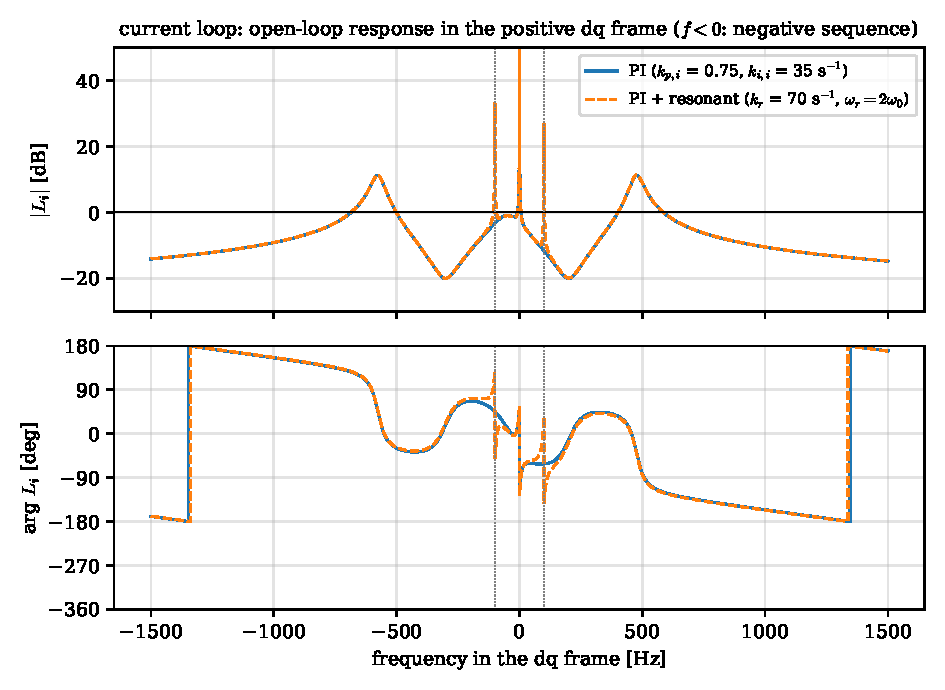
\includegraphics[width=0.95\linewidth]{figures/fig_current_loop_bode.pdf}
\caption{Open-loop response of the current loop of the study model in the positive frame, PI alone and PI with the resonant term at $\pm 2f_0$ (dotted lines). The lobes at about $\pm\SI{550}{Hz}$ are the LCL resonance split by the frame rotation; the phase stays above $\SI{-180}{\degree}$ up to $f_s/6$.}
\label{fig:bode}
\end{figure}

\begin{figure}[htbp]
\centering
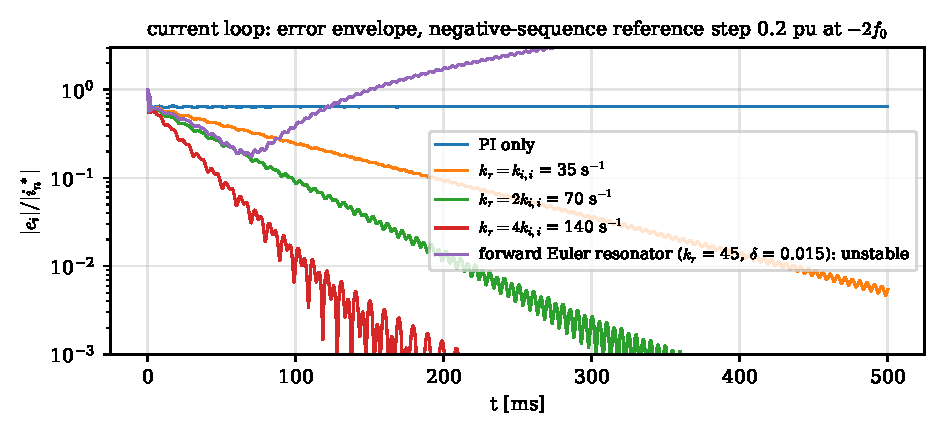
\includegraphics[width=0.9\linewidth]{figures/fig_negseq_tracking.pdf}
\caption{Envelope of the current error for a negative-sequence reference step of \SI{0.2}{pu}: the PI alone keeps a \SI{56}{\percent} error; the resonant term removes it with the rate of Table~\ref{tab:kr}; the forward Euler resonator of the library object diverges.}
\label{fig:tracking}
\end{figure}

\begin{figure}[htbp]
\centering
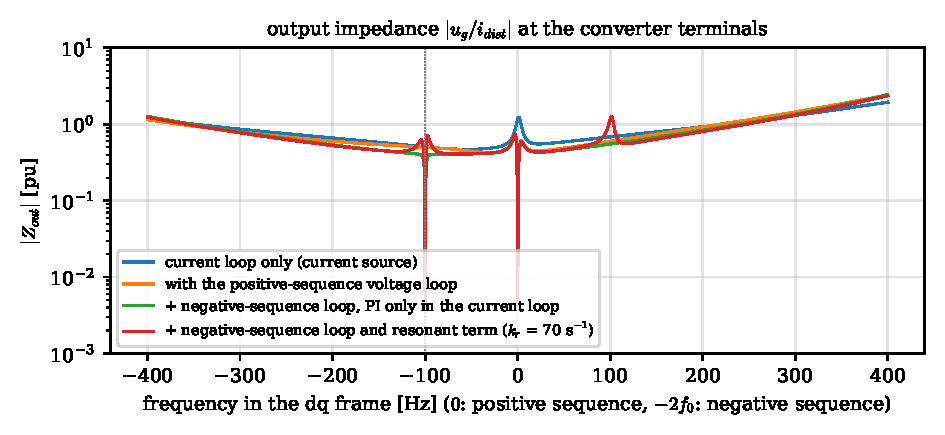
\includegraphics[width=0.9\linewidth]{figures/fig_output_impedance.pdf}
\caption{Output impedance of the converter at its terminals as a function of the frequency in the positive frame: the positive-sequence voltage loop makes it zero at DC (positive sequence), the negative-sequence loop makes it zero at $-2f_0$ (negative sequence); the peak at $+2f_0$ is the lightly damped $+2\wo$ mode of the resonant term.}
\label{fig:zout}
\end{figure}

\begin{figure}[htbp]
\centering
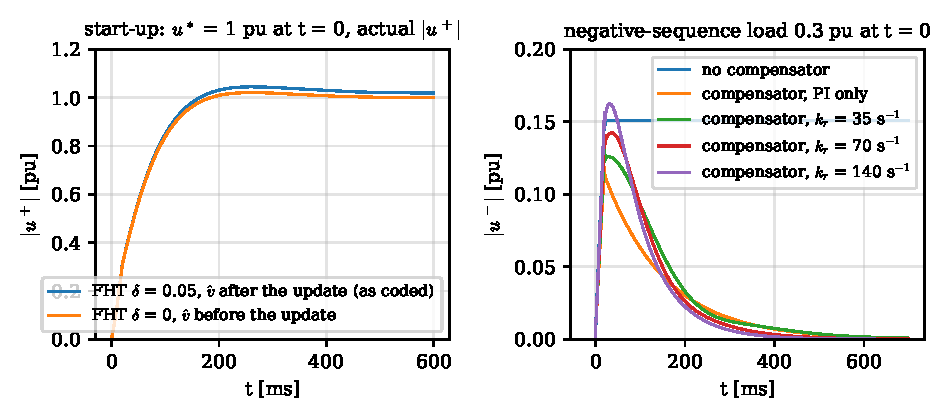
\includegraphics[width=0.9\linewidth]{figures/fig_negseq_load_step.pdf}
\caption{Left: start-up of the terminal voltage (actual positive sequence) with the FHT as coded and with $\delta = 0$ and the same-instant quadrature output: the \SI{1.9}{\percent} offset of Sect.~\ref{sec:disc_fht}. Right: negative-sequence terminal voltage after a negative-sequence load current step of \SI{0.3}{pu}, without the compensator (permanent \SI{0.15}{pu}) and with it, for the PI alone and for three values of $k_r$.}
\label{fig:loadstep}
\end{figure}

\begin{figure}[htbp]
\centering
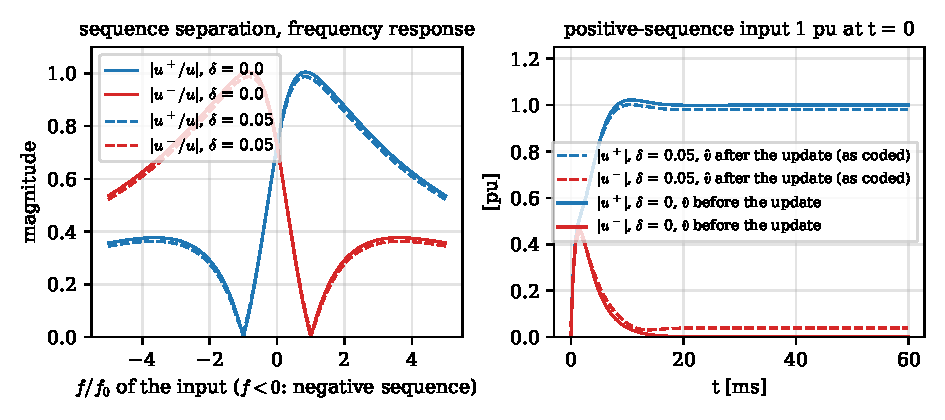
\includegraphics[width=0.9\linewidth]{figures/fig_fht_sequence_separation.pdf}
\caption{FHT sequence separation at \SI{50}{Hz}: frequency response of $\vec u^+/\vec u$ and $\vec u^-/\vec u$ (left, continuous time; exact at $\pm f_0$ for $\delta = 0$) and response to a positive-sequence input applied at $t = 0$ with the discrete observer (right): the estimates settle in \SI{12}{ms}; the coded variant leaves \SI{4}{\percent} in $|\vec u^-|$.}
\label{fig:fht}
\end{figure}

\begin{figure}[htbp]
\centering
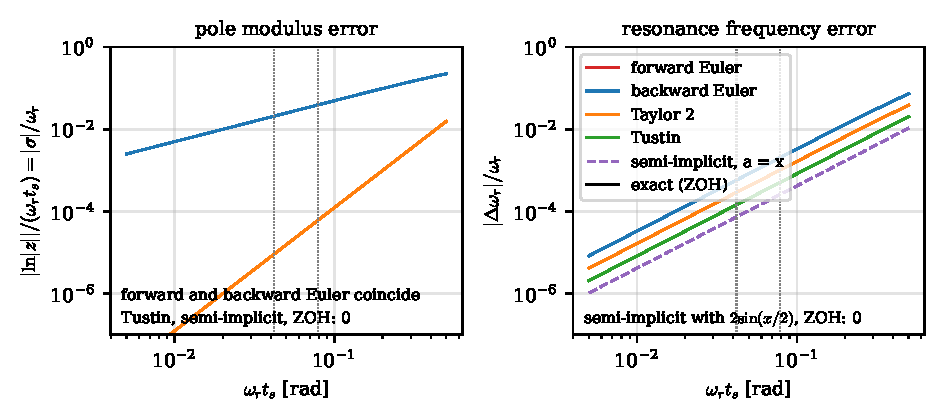
\includegraphics[width=0.9\linewidth]{figures/fig_resonant_discretization.pdf}
\caption{Discretization of the undamped resonant model as a function of $\wres\ts$: apparent damping rate relative to $\wres$ (left) and resonance frequency error (right); the dotted lines mark the two applications (\SI{33.3}{Hz} at \SI{200}{\micro s}, \SI{100}{Hz} at \SI{125}{\micro s}).}
\label{fig:disc}
\end{figure}

Table~\ref{tab:modes} collects the closed-loop modes of the complete model. The resonant term with $k_r = 2\kii$ leaves the margins of the current loop unchanged (modulus margin 0.662 against 0.671), tracks a negative-sequence current reference with zero error (settling \SI{183}{ms}, Fig.~\ref{fig:tracking}) and, in the complete loop, raises the damping of the negative-sequence voltage mode from $-7.3$ to $\SI{-10.4}{s^{-1}}$. The forward Euler resonator is unstable in the current loop and in the complete loop. The FHT with $\delta = 0$ and the same-instant quadrature output removes the \SI{1.9}{\percent} offset of the regulated voltage and the \SI{4}{\percent} spurious negative-sequence estimate without any change of the dynamics.

\begin{table}[htb]
\centering\small
\caption{Complete loop of the study model: least damped modes (frequency in the positive frame, damping rate) and response to a \SI{0.3}{pu} negative-sequence load current.}
\label{tab:modes}
\begin{tabular}{@{}R{3.7cm}R{6.3cm}lc@{}}
\toprule
configuration & least damped modes [Hz, s$^{-1}$] & $|\vec u^-|$ peak, settling & $|\vec u^+|$ \\
\midrule
voltage loop, no compensator & $(-1, -10.8)$, $(+2, -20.4)$, $(-59, -295)$ & \SI{0.15}{pu} permanent & 1.019 \\
compensator, PI only in the current loop & $(-100, -7.3)$, $(-1, -10.6)$, $(+2, -20.5)$ & 0.12, \SI{413}{ms} & 1.019 \\
compensator, $k_r = 35$ & $(-99, -7.3)$, $(+101, -8.7)$, $(-1, -10.6)$, $(-102, -12.4)$ & 0.13, \SI{444}{ms} & 1.019 \\
compensator, $k_r = 70$ & $(-99, -10.4)$, $(-1, -10.6)$, $(+102, -17.6)$, $(+2, -20.5)$ & 0.14, \SI{344}{ms} & 1.019 \\
compensator, $k_r = 140$ & $(-1, -10.6)$, $(-99, -12.8)$, $(+2, -20.5)$, $(+103, -35.6)$ & 0.16, \SI{304}{ms} & 1.019 \\
compensator, $k_r = 70$, forward Euler resonator & $(+102, +8.4)$: unstable & -- & -- \\
compensator, $k_r = 70$, FHT $\delta = 0$, $\vhat$ same instant & $(-99, -10.9)$, $(-1, -11.1)$, $(+102, -17.7)$, $(+2, -20.2)$ & 0.14, \SI{329}{ms} & 1.000 \\
\bottomrule
\end{tabular}
\end{table}

% =====================================================================================================
\clearpage
\section{Parameters}
\label{sec:parameters}

\begin{table}[htb]
\centering\footnotesize\setlength{\tabcolsep}{4pt}
\caption{Control parameters of the two applications (per unit of the converter base).}
\label{tab:param}
\begin{tabular}{@{}llll@{}}
\toprule
 & symbol & VFC0 test bench & study model (\code{grid\_forming\_dq}) \\
\midrule
fundamental, PWM & $f_0$, $f_{pwm}$ & \SI{16.67}{Hz}, \SI{2.5}{kHz} double update & \SI{50}{Hz}, \SI{4}{kHz} double update \\
control period, solver step & $\ts$, $t_c$ & \SI{200}{\micro s}, \SI{1}{\micro s} & \SI{125}{\micro s}, \SI{0.625}{\micro s} \\
base & $u_{bez}$, $i_{bez}$ & \SI{326.6}{V}, \SI{777.8}{A} & \SI{326.6}{V}, \SI{567.0}{A} \\
voltage reference & $u^*_\xi$, $u^*_\eta$ & 1, 0 (\SI{400}{V}) & 1, 0 \\
positive-sequence voltage PI & $\kpu$, $\kiu$, $i_{lim}$ & 0.5, \SI{18}{s^{-1}}, \SI{1.65}{pu} & 0.5, \SI{18}{s^{-1}}, \SI{1.65}{pu} \\
negative-sequence voltage PI & $\kpn$, $\kin$, $i_{n,lim}$ & 0.5, \SI{18}{s^{-1}}, \SI{1.65}{pu} & 0.5, \SI{18}{s^{-1}}, \SI{1.65}{pu} \\
current PI & $\kpi$, $\kii$, $u_{lim}$ & 0.4, \SI{35}{s^{-1}}, 1 & 0.75, \SI{35}{s^{-1}}, 1 \\
resonant term & $\wres$, $k_r$ & $2\wo = \SI{209.4}{rad/s}$, \SI{70}{s^{-1}} & $2\wo = \SI{628.3}{rad/s}$, \SI{70}{s^{-1}} \\
FHT & $\wo$, $\delta$, $L_d$, $t_{reset}$ & \SI{104.7}{rad/s}, 0.05, $[0.100\ \ 5.61]$, \SI{12.5}{ms} & \SI{314.2}{rad/s}, 0.05, $[0.182\ \ 29.6]$ \\
clip release, quantizer & $c_{rel}$, $q$ & \SI{0.001}{s^{-1}}, $2^{-11}$\,pu & \SI{0.001}{s^{-1}}, $2^{-11}$\,pu \\
dead time, duty limits & $t_{dead}$ & \SI{3}{\micro s}, $[0.02, 0.98]$ & \SI{3}{\micro s} \\
master/slave & \code{slave} & 0 (GFM1), 1 (GFM2) & -- \\
\bottomrule
\end{tabular}
\end{table}

The gains of the two voltage loops are equal; the lower proportional gain of the VFC0 current loop ($0.4$ against $0.75$) and the longer control period lower its crossover, and the resonant term keeps $k_r = 2\kii$. The plant-dependent figures of this note (crossover, margins, settling times, output impedance) refer to the study model; the discretization figures (Tables~\ref{tab:disc} and \ref{tab:fht}) are given for both.

% =====================================================================================================
\section{Conclusions}

The controller is a cascade of vector PIs in the positive and in the negative synchronous frame, fed by an FHT that separates the sequences of the terminal voltage, with a resonant term at $2\wo$ in the current loop so that the negative-sequence current reference, a sinusoid at $2f_0$ in the positive frame, is tracked without error. In continuous time the design reduces to three numbers per loop: the crossover of the current loop ($\kpi\kmod/L_1'$, \SI{243}{Hz} for the study model with a \SI{72}{\degree} phase margin), the integrator and resonant poles given by the pole-displacement rule (\ref{eq:pole_rule}), which turns the implemented $k_r = 2\kii$ into equal convergence rates for the positive and the negative sequence ($-18.7$ and $\SI{-19.6}{s^{-1}}$), and the dominant pole of the voltage loops (\ref{eq:voltage_pole}), about $\SI{-11}{s^{-1}}$, which makes the converter a stiff voltage source for both sequences at the fundamental and a soft one above a few hertz. The FHT separates the sequences exactly at $\pm\wo$ for any observer gains provided its internal model is undamped.

In the discrete implementation two internal models must reproduce the frequency of the phase generator exactly. The resonant term does, through the semi-implicit form with $a = 2\sin(\wres\ts/2)$, whose poles are those of the zero-order hold; the forward Euler form of the library object is unstable at \SI{100}{Hz} and \SI{125}{\micro s} and marginal at \SI{16.7}{Hz} and \SI{200}{\micro s}, and must not be used. The FHT reproduces it closely enough with the Taylor matrix of the C code (an exact rotation matrix would cost the same), but two details of the implementation are worth \SI{2}{\percent} each in the sequence separation and \SI{1.9}{\percent} in the regulated voltage: the damping $\delta = 0.05$ of its internal model and the quadrature output taken one step after the in-phase one. Setting $\delta = 0$ and reading both outputs at the same instant removes both at no cost. The PI integrators, the frame rotations and the limiters need no special care.

% =====================================================================================================
\begin{thebibliography}{99}
\small
\bibitem{fortescue1918} C.~L. Fortescue, ``Method of symmetrical co-ordinates applied to the solution of polyphase networks,'' \emph{Trans. AIEE}, vol.~37, part~II, pp.~1027--1140, 1918.
\bibitem{harnefors2007} L.~Harnefors, ``Modeling of three-phase dynamic systems using complex transfer functions and transfer matrices,'' \emph{IEEE Trans. Ind. Electron.}, vol.~54, no.~4, pp.~2239--2248, Aug. 2007.
\bibitem{buso2015} S.~Buso and P.~Mattavelli, \emph{Digital Control in Power Electronics}, 2nd ed. Morgan \& Claypool, 2015.
\bibitem{parker2014} S.~G. Parker, B.~P. McGrath, and D.~G. Holmes, ``Regions of active damping control for LCL filters,'' \emph{IEEE Trans. Ind. Appl.}, vol.~50, no.~1, pp.~424--432, Jan./Feb. 2014.
\bibitem{holmes2009} D.~G. Holmes, T.~A. Lipo, B.~P. McGrath, and W.~Y. Kong, ``Optimized design of stationary frame three phase AC current regulators,'' \emph{IEEE Trans. Power Electron.}, vol.~24, no.~11, pp.~2417--2426, Nov. 2009.
\bibitem{zmood2003} D.~N. Zmood and D.~G. Holmes, ``Stationary frame current regulation of PWM inverters with zero steady-state error,'' \emph{IEEE Trans. Power Electron.}, vol.~18, no.~3, pp.~814--822, May 2003.
\bibitem{teodorescu2006} R.~Teodorescu, F.~Blaabjerg, M.~Liserre, and P.~C. Loh, ``Proportional-resonant controllers and filters for grid-connected voltage-source converters,'' \emph{IEE Proc. Electr. Power Appl.}, vol.~153, no.~5, pp.~750--762, Sept. 2006.
\bibitem{liserre2006} M.~Liserre, R.~Teodorescu, and F.~Blaabjerg, ``Multiple harmonics control for three-phase grid converter systems with the use of PI-RES current controller in a rotating frame,'' \emph{IEEE Trans. Power Electron.}, vol.~21, no.~3, pp.~836--841, May 2006.
\bibitem{yepes2010} A.~G. Yepes, F.~D. Freijedo, J.~Doval-Gandoy, O.~L\'opez, J.~Malvar, and P.~Fernandez-Comesa\~na, ``Effects of discretization methods on the performance of resonant controllers,'' \emph{IEEE Trans. Power Electron.}, vol.~25, no.~7, pp.~1692--1712, July 2010.
\bibitem{rodriguez2006} P.~Rodr\'iguez, R.~Teodorescu, I.~Candela, A.~V. Timbus, M.~Liserre, and F.~Blaabjerg, ``New positive-sequence voltage detector for grid synchronization of power converters under faulty grid conditions,'' in \emph{Proc. IEEE PESC}, Jeju, 2006, pp.~1--7.
\bibitem{song1999} H.-S. Song and K.~Nam, ``Dual current control scheme for PWM converter under unbalanced input voltage conditions,'' \emph{IEEE Trans. Ind. Electron.}, vol.~46, no.~5, pp.~953--959, Oct. 1999.
\bibitem{rodriguez2007} P.~Rodr\'iguez, J.~Pou, J.~Bergas, J.~I. Candela, R.~P. Burgos, and D.~Boroyevich, ``Decoupled double synchronous reference frame PLL for power converters control,'' \emph{IEEE Trans. Power Electron.}, vol.~22, no.~2, pp.~584--592, Mar. 2007.
\bibitem{savaghebi2012} M.~Savaghebi, A.~Jalilian, J.~C. Vasquez, and J.~M. Guerrero, ``Secondary control scheme for voltage unbalance compensation in an islanded droop-controlled microgrid,'' \emph{IEEE Trans. Smart Grid}, vol.~3, no.~2, pp.~797--807, June 2012.
\bibitem{rocabert2012} J.~Rocabert, A.~Luna, F.~Blaabjerg, and P.~Rodr\'iguez, ``Control of power converters in AC microgrids,'' \emph{IEEE Trans. Power Electron.}, vol.~27, no.~11, pp.~4734--4749, Nov. 2012.
\bibitem{teodorescu2011} R.~Teodorescu, M.~Liserre, and P.~Rodr\'iguez, \emph{Grid Converters for Photovoltaic and Wind Power Systems}. Wiley-IEEE Press, 2011.
\bibitem{franklin1998} G.~F. Franklin, J.~D. Powell, and M.~L. Workman, \emph{Digital Control of Dynamic Systems}, 3rd ed. Addison-Wesley, 1998.
\end{thebibliography}

\end{onehalfspace}
\end{document}
